\documentclass[a4paper,11pt]{ltjsarticle}
% 基本とドライバ関連
\usepackage{graphicx}
\usepackage{xcolor}
\usepackage{makeidx}
\usepackage{ascmac}

% LuaTeX-ja設定
\usepackage{luatexja}% 日本語したい
\usepackage[haranoaji,no-math,deluxe,expert,nfssonly,match,scale=1.0]{luatexja-preset}
\renewcommand{\kanjifamilydefault}{\gtdefault}% 既定をゴシック体に
\usepackage{lltjext}

% 数式系基本
\usepackage{amsmath}
\usepackage{amsthm}
\usepackage{amssymb}
\usepackage{mathtools}
% \mathtoolsset{showonlyrefs=true}
\usepackage{derivative}
\usepackage[b]{esvect}
\usepackage{nicematrix}
\usepackage{siunitx}
\usepackage{bm}

% 画像関係
\usepackage{animate}
\usepackage{svg}
\usepackage{tikz}

%表関連
\usepackage{multirow}

% 自然科学用追加
% \usepackage{chemmacros}
% \usechemmodule{all}
% \selectchemgreekmapping{fontspec}
\usepackage{chemfig}
\setchemfig{atom sep=1.5em}
% \ifdraft{}{\setchemfig{bond join=true}}

% 数式フォント設定
\usepackage{anyfontsize}
\newcommand{\sfscale}{0.98}
\newcommand{\ttscale}{0.96}
% \usepackage[mathnoalias]{iwona}
% % \setmainfont{Iwona}
% \usepackage[scale=\sfscale]{roboto}
% \usepackage[scale=\ttscale]{roboto-mono}
% \usepackage{BOONDOX-uprscr}
% \usepackage{BOONDOX-ds}

% ページ設定
\usepackage{geometry}
\geometry{left=25truemm, right=25truemm, top=25truemm, bottom=25truemm}
% \pagestyle{empty}

% hyperref関連
\usepackage{bookmark}
\usepackage{xurl}
\hypersetup{unicode,bookmarksnumbered=true,colorlinks=true,final}

%%%%%%%%%%%%%%%%%%%%%%%
\graphicspath{{../figure/}{../../figure/}}


\usepackage{bm}


%微分関連のマクロ
%
\newcommand{\diff}{\mathrm d}
\newcommand{\difd}[2]{\dfrac{\diff #1}{\diff #2}}
\newcommand{\difp}[2]{\dfrac{\partial #1}{\partial #2}}
\newcommand{\difdd}[2]{\dfrac{\diff^2 #1}{\diff #2^2}}
\newcommand{\difpp}[2]{\dfrac{\partial^2 #1}{\partial #2^2}}

\allowdisplaybreaks[3]

\title{高分子モデルを理解する。\\ミクロな化学的視点から、粗視化した物理的視点へ}
\author{佐々木裕 \thanks{e-mail: hiroshi\_sasaki$@$mail.toagosei.co.jp}}
\date{\today}

\begin{document}
\maketitle

\setcounter{tocdepth}{2}
\pagenumbering{roman}
\tableofcontents

\newpage

\setcounter{secnumdepth}{3}
\pagenumbering{arabic}

% \section*{はじめに}

% 高分子を用いた材料は、金属や木材などの古くから使われてきている材料とは異なる特性を有する機能性材料として各種分野で大量に使用されています。
% そして、今後もますますその使用量および適応分野は増加していくものと期待されています。

% このメモは、おもに有機化学をベースにした合成化学的なアプローチで高分子を取り扱ってきたような化学系研究者を対象として作成しました。
% すなわち、有機合成的にモノマーの化学構造を意識して、重合反応により生成したポリマーをモノマーユニットの繰り返した化合物として取り扱い、その物性については他の物性系の研究者と共同研究することで丸投げしてしまいがちな方たちに向けてまとめたわけです。

% 高分子を材料として使いこなしていくためには、高分子を化学的に合成するだけではなく、その特徴や性質を高分子物理という考え方で整理していく物理的なアプローチも必要となります。
% しかしながら、高分子物理のテキストは物理系の学生を対象としている場合が多く、モノマーの化学構造のようなミクロな描写を無視した粗視化した表現として、高分子鎖を紐のようなものとして取り扱います。
% そして、そのような紐の一般的な性質について議論を進めていくために、最初の数ページから、数学、統計、熱力学、統計力学等の基礎知識が必要となるような記述が出てくることがよくあります。
% 数学の得意でない化学系の学生は、このイントロの時点で躓いてしまうわけです。

% このメモは、高分子物理の内容をきちんと理解できることを目的として、高分子物理のはじめの一歩ぐらいに対応する非常に初歩的な事項である「粗視化した高分子モデル」について、ゆっくりと理解できるように意図しています。
% まず、高分子材料の機能を発現させる際に、ミクロとマクロをつなぐメゾスケールが重要であることを確認します。
% その認識に立って、化学者になじみやすいミクロな化学構造を用いて高分子鎖の細長い紐のようなイメージを概観した後に、各種の高分子モデルについて示します。
% 最後に、粗視化したメゾスケールでの高分子の大きさについての議論を行います。
% %最後に、高分子の特徴的なふるまいについて統計力学的な見方で理解を深めたいと考えています。

% なお、数学アレルギーの方を考慮して、できるだけ本文中では数学的な表現を少なくしました。
% そして、数式を取り入れた細かい説明は付録にまとめました。

% 残念ながら、この程度の知識を付けたからといってすぐに役立つわけではないのですが、これまでに学んできた「化学の見かた」に「物理のやり方」を加えていくための最初の一歩となればよいなと期待しております。

%できれば、参考文献に目を通していただければと思いますが、強制は致しません。
%ただし、\pageref{homework} ページの「アンケート」だけは、{\bf 必ず記述、提出}してください。

\thispagestyle{empty}
\newpage

\setcounter{page}{1}
\section{メゾスケールと高分子の形}

% ここでは、有機化学者が化学式を用いて構造を考えるような比較的分子量の低い分子(たとえば、モノマー単位に対応)の微小(ミクロ)な大きさのイメージと、実際に高分子材料を手に取って使用するような大きさ(マクロ)との間にある、中間的な大きさに対応する「メゾスケール」という考え方から始めていきましょう。

% その議論の後に、高分子の形についても簡単に触れます。

% \subsection{ミクロとマクロ}

% 有機化学で対象とする炭素系の分子において基本的な長さとなる炭素結合は、\qty{1.54}{\angstrom} $\simeq$ \qty{10e-1}{\nano\meter}10^{-1} 程度の長さです。
% したがって、化学式で全構造を書けるような低分子の化学構造をベースに考えているということは、たかだか 1 nm 程度の微小な大きさで物質を捉えていることになります。
% 実際、有機合成のような分野においては、このような考え方で十分な場合がほとんどなのでしょう。
% 大きさを測る基準となる物差しという意味でスケールという言葉を使って、対照としている物質の大きさを表すことにしましょう。
% 原子をあらわに見るようなこの程度の大きさに関する議論をミクロスケールと呼びます。

% 一方、我々が目に見えて実感できるのは、\qty{1}{\mm}程度以上の大きさでの事象となっています。
% たとえば、身の回りに多数存在するプラスティック材料の強さを表す力学特性のような理解しやすい機能というものは、一般に、手で触って実感できるような大きさで発現するものです。
% このような大きさでの議論をマクロスケールと呼び、

% したがって、材料の各種機能を調べて使いこなすということは、マクロな大きさでの評価を用いる場合が多いことになります。

% このことを一般的な言葉にしてみれば、「木を見て森を見ず」\footnote{余談になりますが、宇宙、銀河の大きさから原子核の大きさに至るまでのとんでもないスケール(尺度)をなんとなくイメージできるサイトを株式会社 Nikon が作っています。
% 	\url{https://www.jp.nikon.com/company/corporate/sp/universcale/scale.html}
% 	これは一見の価値があると思います。
% }

% \subsection{メゾスケール}

% したがって、マクロな大きさで機能を有する材料の設計を行う際には、化学的な感覚でナノスケールの大きさで設計することと、実際に評価しているマクロスケールとの間にある、長さの次元で $10^6$ にも及ぶ「メゾ(中間的)スケール領域」をきちんと取り扱うことの、両方が重要になってくるわけです。
% ただし、対象とする機能に応じて、このメゾスケールの振る舞いの重要性は異なってきます
% \footnote
% {
% 例えば、一般に光学特性のような分子構造に強く依存する特性はミクロな議論が主となる場合が多く、自動車タイヤの力学特性のようなマクロよりな特性の場合はメゾスケールでの階層構造が非常に重要であることが知られてきている。
% }。

% 高分子の場合、このメモで示すように、その鎖としての構造の自由度が非常に高く、マクロな機能性へのメゾスケール構造の寄与が非常に大きいことが知られています。
% このことが、低分子には見られない高分子特有の振る舞いの原因であり、このような高分子の形状に起因した特徴的な振る舞いをうまく利用して材料設計を行おうという考えが、近年、急速に広まってきています
% \footnote
% {
% このような流れの端緒は、ノーベル賞受賞者であるド・ジャンによるものであり、金属のように硬い物質との対比で、「ソフトマター」と名付けられています。
% ソフトマターの対象となるのは、高分子だけではなくて、界面活性剤が形成するミセルやビヒクルのようなものも含まれており、決して、分子量が大きいことが必須なわけではありません。

% 一般にソフトマターと呼ばれるものは、各種の構造間の遷移に伴う活性化エネルギーが熱エネルギー程度($\simeq k_B T$)であり、構造変換が容易に起こるような、ソフトな(移ろいやすい)物質あるいは事象を指しています。
% }。
% \subsection{高分子の形}

% 高分子の形を考える場合に、立体配置(コンフィギュレーション)と立体配座(コンフォメーション)という、2つの異なった観点で考える必要がある。

% 立体配置は、モノマー内あるいはモノマー間の共有結合の生成により規定される構造の様式であり、主として以下の3つのような結合様式に基づいている
% \vspace{-2mm}
% \begin{itemize}
% \item 
% 頭-尾、頭-頭結合
% \item
% 幾何異性体
% \item
% 立体規則性(光学異性体)
% \end{itemize}
% \vspace{-2mm}
% さらには、高分子鎖の主鎖の分岐やデンドリマー、環状構造のような大きなスケールの構造も含まれてくる。
% いづれにせよ、構造の大きさにかかわらず、共有結合を切断することなしには異なる構造へと遷移できないものである。
% 一般に、合成系研究者にとっての高分子の設計とは、この立体配座を主に考えている場合が多いようである。

% 一方、立体配座は、第二章に示すように、高分子鎖中の C-C 結合周りの回転に基づくものであり、一般に、熱揺らぎ程度で容易に遷移してしまうものである。
% したがって、単一の構造として捉えることは困難となり、統計的な手法で評価する必要が生じることになる。

% 立体配置は、適切な記述方法を選択すれば、化学構造式としての認識も容易に行えるのであるが、立体配座のほうは、化学構造式としては書き表すことが困難であり、実感することが困難なものである。
% しかしながら、後述するように、この立体配座こそが高分子の膨大な内部自由度を生み、高分子材料の特徴的な機能発現に大きく寄与するものである。

% \subsection{章末問題}

% 	\begin{enumerate}
% 		\item
% 		(メゾスケール)\\
% 		メゾスケールのことについて、できるだけ自分の言葉で説明してみてください。
% 		\item
% 		(高分子の形)\\
% 		高分子の形について、立体配置(コンフィギュレーション)と立体配座(コンフォメーション)という言葉を意識して、説明してください。
% %		(ヒント)\\
% %		C-C 結合の結合長が 1.54 \AA、三つの炭素が形成する C-C-C 結合が約 $109.5^o$ の結合角ということを考慮して、平面ジグザグ構造でのモノマー二つ分の絵を書いてみれば、
% %		ポリマー鎖の伸長方向とそれに垂直な方向との長さが見積れます。

% 	\end{enumerate}
\newpage

\section{高分子鎖のイメージ}

高分子鎖は、模式的には、「非常に細くてとても長い紐が、くるくると丸まったもの」と表現され、「このような高分子鎖の形状に起因して、低分子とは大きく異なった高分子に特有な振る舞いを示す」とされている。
高分子を使いこなして特徴ある機能を発現できる材料とするためには、高分子に特有の形状をきちんと理解することが必須となるわけである。

このような高分子のイメージについて、まず、ミクロな化学構造の結合状態をみることから始めて、少しずつ理解してみよう。

\subsection{細くて長い}

高分子の例として、メチレンを繰り返し単位とした連鎖からなる最も単純な構造であるポリエチレンを対象として考えてみよう。

そのポリマーの構造は、エチレンモノマー単位が重合により多数連結した鎖であり、それぞれのモノマー単位は C-C 結合でつながっている。
なお、C-C 結合の結合長は 1.54 \AA で、三つの炭素が形成する C-C-C 結合は約 $109.5^o$ の結合角を有している
\footnote
{
炭素原子が正四面体の重心に来るようにおいた場合に、その四つの結合のそれぞれが正四面体の頂点となるような構造を取っていることから、この結合角は理解できる。
なお、炭素の立体構造は以下である。
\begin{center}
	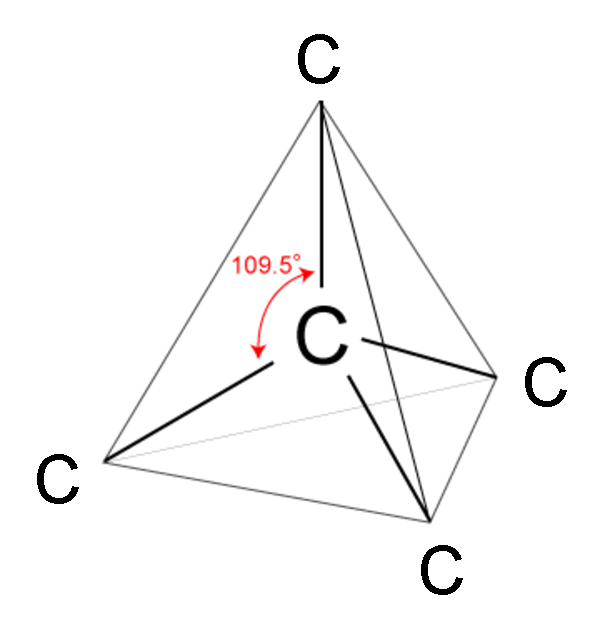
\includegraphics[width=2.5cm]{carbon.eps}
\end{center}

この結合角の具体的な導出については、 \ref{sec: carbon_BA} に示した。
}。

ここで、ポリマーの主鎖のモデルとして、まず、炭素が四個のアルキルであるブタンを考えてみよう。
真ん中の炭素結合(2 位の炭素と 3 位の炭素との間の結合:CH$_3$-CH$_2$\colorbox{gray}{-}CH$_2$-CH$_3$)に対して、ニューマン投影式を考えると、エネルギーの低い状態として、それぞれのメチル基がトランスの位置
\footnote
{
トランス配座は、最初の三つの炭素の張る平面上で 1 位の炭素と 4 位の炭素が反対の位置(トランス)となる状態であり、ポテンシャル・エネルギーが最低となる。
}
と、ゴーシュの位置
\footnote
{
ゴーシュ配座は、トランスの位置からみて、回転角 $\phi = \pm 60^o$ に 4 位の炭素が位置する、局所的にエネルギー極小となる状態である。
この場合、1,4 位の炭素の相互作用が存在するため、トランス状態よりはエネルギーは高い。
}
になる状態を想定できることになる。
この時のエネルギー状態図も併せて、以下に示した。
\begin{figure}[htb]
 \centering
	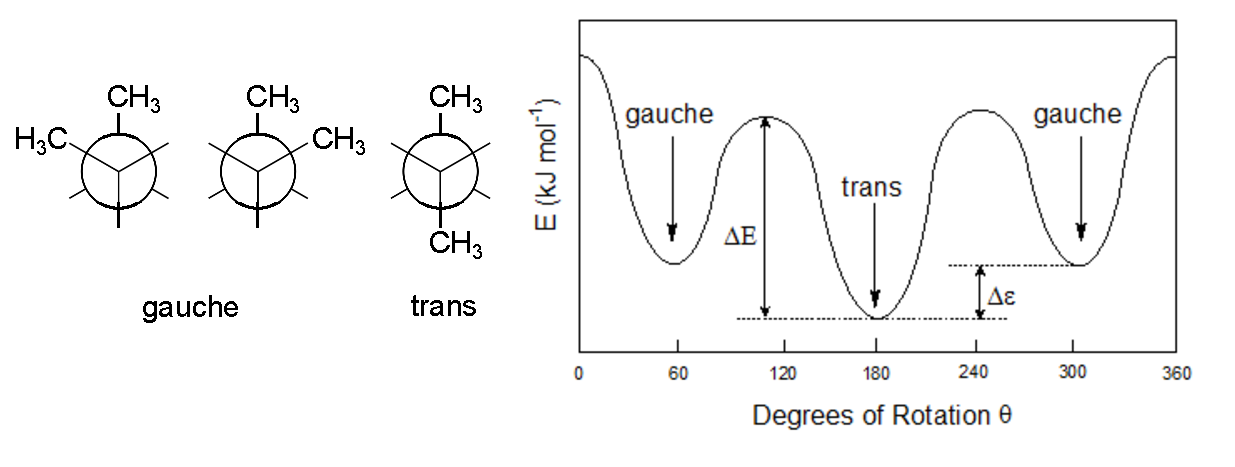
\includegraphics[width=10cm]{butane.eps}
	\caption{ブタンの配座とエネルギー状態図}
	\label{fig: butane}
\end{figure}

ブタンのモデルをベースに考えると、ポリマー主鎖は、ブタンの両端のメチル基の位置からさらに結合が伸びているものとモデル化して考えることができる。
ここで、熱的に安定な状態(よりエネルギーの低いトランス状態)の極限として主鎖の炭素が全部トランスの配置にある状態を考えると、ポリマー鎖は一つの平面上にジグザグに伸びた形(平面ジグザグ構造)となる。

簡便のために、水素を無視して、C-C 結合(結合長は 1.54 \AA)のみを考えてみよう。
このとき、ポリエチレンの直径は約 0.09 nm、また、ポリマー鎖中のモノマー単位の長さは約 0.25 nm と見積もることができる(章末問題 \ref{it:2-1})。
そして、このようなモノマー単位が、仮に、平面ジグザグ構造の連鎖として直線的につながったと考えると、例えば、ポリエチレンの分子量が 10 万であった場合には、その長さは約 900 nm となる
\footnote
{
この時、縦横比を表すアスペクトレシオを考えると、10000 ということになる。
}(章末問題 \ref{it:2-2})。

もっと手に取って扱えるような大きさで考えてみよう。
このヒモを直径 5 mm のチョークを使って横一本の線で黒板に書いたとすると、その長さは約 50 m (普通の黒板の 10 枚分程度)ということになる。
いかに高分子が細長い形状をしているかが想像できるであろう。
 


\subsection{くるくる丸まる}

高分子をピンと引き延ばすと、非常にアスペクト比の高い細長いものとなることを、上に示した。
しかしながら、自然な状態での実際の高分子は、決してこのような伸び切り構造を取っているわけではない。
ぐるぐるに丸まった、ランダムコイルと呼ばれる状態になっていることが知られている。
このことを、統計力学的な考え方で確かめてみよう。

統計力学によれば、エネルギーの異なる二つの状態(エネルギー差 $\Delta E$)の出現確率の比 $r(\Delta E)$ は、ボルツマン因子を用いて、下式のように表すことができる
\footnote
{
ボルツマン因子とは、温度 $T$ の熱平衡状態にある系において、エネルギー $E_i$ である状態 $i$ が出現する相対確率 $P(E_i)$ を、下式のように定める重み因子である。
ボルツマン因子は、通常カノニカル分布によって記述される系を議論する際に用いられる。
\begin{align*}
P(E_i) = \dfrac{1}{Z} \exp(-\beta E_i)
\end{align*}
ここで、$Z=\sum_i \exp(-\beta E_i)$ は、$\sum_i P_i = 1$ とするための規格化因子であり、分配関数、あるいは、状態和と呼ばれる。

}(章末問題 \ref{it:2-3})。
\begin{equation}
r(\Delta E) = \exp(-\beta \Delta E)=\exp \left( -\dfrac{\Delta E}{k_B T} \right)
\label{eq:ratio}
\end{equation}

ただし、$\beta=\dfrac{1}{k_B T}$、$k_B$ はボルツマン定数($k_B =1.380 \times 10^{-23} {\rm J K}^{-1}$)、$T$ は絶対温度である。

このことを利用すれば、前述のトランスとゴーシュ状態とのポテンシャル・エネルギー差 $\Delta \varepsilon$ に基づいて、熱平衡状態でのそれぞれの状態の出現確率の比を求めることができる。
トランス状態が連続する限り、ポリマー鎖は平面ジグザグ構造により直線的に伸びていくが、ゴーシュが出現することで鎖の曲りが生じる。
一般に、このエネルギー差 $\Delta \varepsilon$ は数 kJ mol$^{-1}$ 程度であるので、数個程度のモノマー単位の連鎖ごとに、ゴーシュ状態が出現、すなわち、ポリマー主鎖が曲ることになる(章末問題 \ref{it:2-4}、\ref{it:2-5})。

前述のように、ポリマー鎖は非常に細長いものであるから、10個以下の連鎖で少し曲がるような程度の曲りであっても、全体でみれば、くるくると丸まったものとなっていることが理解できる。

\subsection{ぐにゅぐにゅと蠢く}

さらに、トランス状態からゴーシュ状態へと遷移する際のエネルギー障壁($\Delta E$)を用いた考察から、この遷移の起こる頻度を見積もることも可能である。
分光学的な測定から、ブタンにおける C-C 結合周りの回転振動数は、$10^{12}$ sec$^{-1}$ のオーダーで生じることが知られている。
トランス $\leftrightarrow$ ゴーシュの相互遷移のエネルギー障壁は $10 \sim 20$ kJ mol$^{-1}$ 程度であるので、ボルツマン因子を用いて評価すると、室温での遷移は $10^{9}$ sec$^{-1}$ 程度のオーダーで生じるものと見積もることができる(章末問題 \ref{it:2-6})。

実際の高分子においては、主鎖周りの影響を受けるため、この回転運動の振動数は低いものとなり、また、エネルギー障壁も大きくなると考えられる。
しかしながら、それでも十分に高い頻度でこのような回転異性化によるコンフォメーションの変化が生じるであろうということが想像できる。
このような変化が、高分子のミクロブラウン運動と呼ばれる運動モードの起源の主要なひとつである。

\subsection{章末問題}

	\begin{enumerate}
		\item
		\label{it:2-1}
		(モノマー単位の大きさの見積もり)\\
		文中に示したポリエチレンの平面ジグザグ構造に基づく伸び切り構造の大きさの見積もりを、具体的に説明してください。\\
		(ヒント)\\
		C-C 結合の結合長が 1.54 \AA、三つの炭素が形成する C-C-C 結合が約 $109.5^o$ の結合角ということを考慮して、平面ジグザグ構造でのモノマー二つ分の絵を書いてみれば、
		ポリマー鎖の伸長方向とそれに垂直な方向との長さが見積れます。

		\item
		\label{it:2-2}
		(伸び切り鎖の長さの見積もり)\\
		ポリエチレンの分子量が 10 万であった場合に、その平面ジグザグ構造の伸び切り鎖の長さが約 900 nm となることを、具体的に説明してください。\\
		(ヒント)\\
		分子量が 10 万であった場合に、その重合度がいくつであるかを算出すればいいだけです。

		\item
		\label{it:2-3}
		(出現確率の比)\\
		エネルギーの異なる二つの状態(エネルギー差 $\Delta E$)の出現確率の比 $r(\Delta E)$ が以下の式となることを説明してください。
		\begin{equation*}
		r(\Delta E) = \exp(-\beta \Delta E)=\exp \left( -\dfrac{\Delta E}{k_B T} \right)
		\end{equation*}
		(ヒント)\\
		熱平衡状態であるカノニカル分布において、エネルギー準位が $E_i$ である状態 $i$ の出現確率 $P(E_i)$ は、下式で表されることを使って、
		二つのエネルギー状態の比を取ってください。\\
		なお、指数関数同士の割り算は、指数の引き算となります。
		\begin{align*}
		P(E_i) = \dfrac{1}{Z} \exp(-\beta E_i)
		\end{align*}

		\item
		(鎖の曲り方の具体例)\\
		以下の二つのクイズを考えてください。

		\begin{enumerate}
			\item
			\label{it:2-4}
			(ポリエチレンの例)\\
			室温($27^o$C)のポリエチレンで、トランスとゴーシュとのポテンシャル・エネルギー差 $\Delta \varepsilon$ が 2.1 kJ mol$^{-1}$ であったとした場合、
			トランス連鎖はどのぐらい続くと見積もればいいことになるでしょうか。\\
			(ヒント)\\
			(\ref{eq:ratio})式に、上記のエネルギー差を入れれば、それぞれの状態の出現確率の比が求まります。
			なお、$k_B \simeq 1.4 \times 10^{-23} {\rm J K}^{-1}$ です。 

			\item
			\label{it:2-5}
			(持続長)\\
			このメモでは詳細に立ち入りませんが、高分子鎖の曲がりやすさを考慮したモデルとして、ミミズ鎖(Worm-like chain)と呼ばれるものがあります。
			このモデルにおいては、粗視化した単位として、モノマー単位が平面ジグザグ構造でまっすぐにつながる長さを統計的に見積もって、
			「持続長 $l_p$」と呼ぶものを使います。\\
			持続長は、以下の表式で表すことができます。
			\begin{equation*}
			l_p = l_0 \exp \left( - \dfrac{\Delta \varepsilon}{k_B T} \right)
			\end{equation*}
			ここで、$l_0$ はモノマー単位の長さであり、ポリエチレンの場合は、C-C 結合の結合長 1.54 \AA を用います。\\
			この式を用いて、上記のポリエチレンの場合の持続長を求めてください。\\
			(ヒント)\\
			結局、統計的に見てトランス連鎖が続く状態を考えて、その具体的な長さを見ているだけです。
	\end{enumerate}
	\item
	\label{it:2-6}
	(トランス・ゴーシュの遷移)\\
	ブタンにおける C-C 結合周りの回転振動数は、$10^{12}$ sec$^{-1}$ のオーダーで生じるとして、トランス $\leftrightarrow$ ゴーシュの相互遷移のエネルギー障壁が、
	15 kJ mol$^{-1}$ 程度であるとした場合、室温での遷移の頻度を見積もってください。
\end{enumerate}

\newpage

\section{粗視化モデルによる高分子の認識}
\label{sec:CG_model}

前章で、高分子鎖の振る舞いについてミクロな化学的視点からスタートして考察し、非常に細長い紐が丸まっているというイメージを持つことができた。
このイメージを、材料としての特性と関連付けていくためには、この「丸まった紐のかたまり」を、何らかの形で定義する必要がある。

前章において、各ボンドがトランス配座を取り直線状に伸びた場合の伸び切り構造の長さという一つの特徴長さについての議論は既に行った。
ここでは、丸まった紐を記述するために、丸まった状態での長さを決めていく方法について確認しよう。
%長さが決まれば、そのかたまりの占める空間の体積はその長さの三乗程度で見積もることができるようになる。

最初に、両末端の距離について考察を行う。
セグメントが目に見えるようなモデルで考えるには、このような長さは便利であるが、実際にはこの長さを実測することは困難である。
続いて、実測が容易である慣性半径という重心からの距離に対応するような長さについての考察を行い、末端間距離との関係を確認する。
なお、前章で示したようなミクロな構造を考慮していたのでは、自由度が大きすぎて議論が困難であるので、大胆に粗視化した自由連結鎖というモデルを用いてスタートすることになる。
モデルの妥当性とついての議論を行った後、最後に、高分子物理で取り扱いが容易であるガウス鎖というモデルについて簡単に説明する。

%\subsection{空間的な大きさの各種モデル}
%

%しかしながら、前述のように、単純な回転異性体モデルでも、その取りうる場合の数は分子量の増加に伴い指数関数的に増加するので、その厳密な取り扱いは非常に困難になる。
%したがって、さらに簡易化した統計的なモデルとして取り扱う必要がある。

\subsection{高分子鎖の大きさ}

ここでは、実在の高分子のモノマー連鎖のことは一旦忘れて、セグメントという球が、長さ $a$ のボンドで連結しているという仮想的なモデルを考えよう。
なお、セグメントは、自由に折れ曲がることのできる単なる結節点として取り扱い、その体積は考えないこととする
\footnote
{
このモデル化の妥当性についても、きちんと議論できるのであるが、ここでは天下りにこういうモデルでの記述できるということにしていただきたい。
}。
このようなモデルは、「自由連結鎖」、あるいは、「ランダム・フライト・モデル」と呼ばれる。

さらに、簡単のために、直鎖上のポリマーを対象として、$N+1$ 個のセグメント(一方の端から、0, 1, $\cdots$, N と番号を付ける)が、$N$ 本のボンドにより一本の紐のように連結していることとする。

以下に、1000 個のセグメントからなる自由連結鎖を二次元平面上に記述した例を示した
\footnote
{
この図は、一方の端のセグメントから単位長さのボンドをランダムに発生させ、次々とつなげて作成したものである。
自由連結鎖のように一定長さのボンドベクトルを任意の方向に発生させるためには、三角関数をうまく使えばよい。(章末問題 \ref{it:3-1})
}。
\begin{figure}[htb]
	\begin{center}
		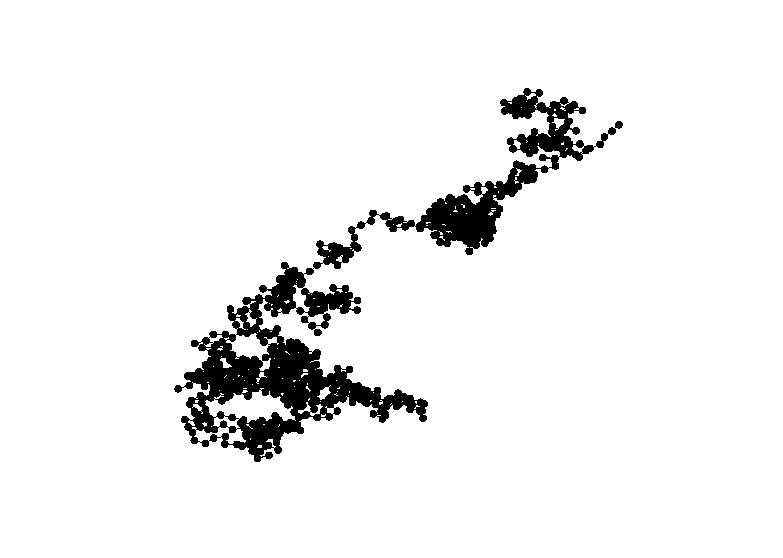
\includegraphics[width=10cm]{RF.eps}
		\caption{自由連結鎖の例(1000 セグメント)}
		\label{fig: RF}
	\end{center}
\end{figure}

自由連結鎖モデルを用いて、「末端間距離」および「慣性半径」という二つの長さについて考えてみよう。

\subsubsection{末端間距離 $R$}

これは、鎖の両末端のセグメント(0 番目と $N$ 番目)との間にベクトル $\bm{R}$ を考え、その二乗の平均 $\langle |\bm{R}|^2 \rangle$ (平均二乗末端間距離)を用いて、下式で定義されるものである(章末問題 \ref{it:3-2})。
\begin{equation}
R=\sqrt{\langle |\bm{R}|^2 \rangle}
\end{equation}

前述の自由連結鎖の例における末端間ベクトルを以下に図示した。
\begin{figure}[htb]
	\begin{center}
		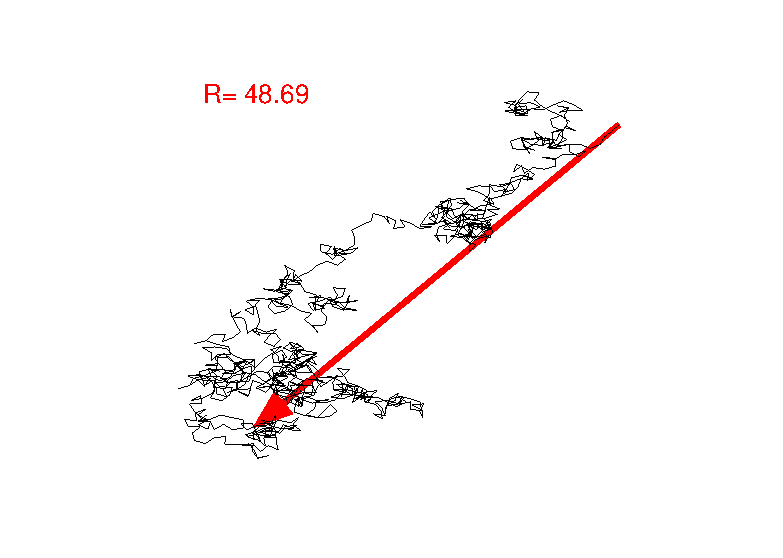
\includegraphics[width=10cm]{RF_EV.eps}
		\caption{末端間ベクトルの例}
		\label{fig: RF_EV}
	\end{center}
\end{figure}

このモデルにおいて、ボンドが自由に連結しているという性質を用いることにより、末端間距離は、以下のように求めることができる。
\begin{align}
R^2
	&= \langle |\bm{R}|^2 \rangle \notag \\
	&=\langle |\bm{r}_0 - \bm{r}_N|^2 \rangle \notag \\
	&=\langle |(\bm{r}_1 - \bm{r}_0) + (\bm{r}_2 - \bm{r}_1) + \cdots + (\bm{r}_N - \bm{r}_{N-1})|^2 \rangle \notag \\
	&=\langle |\bm{u}_0 + \bm{u}_1 + \cdots + \bm{u}_{N-1}|^2 \rangle \notag \\
	&=\left\langle \left|\sum_{i=0}^{N-1}\bm{u}_i \right|^2 \right\rangle \notag \\
	&= 
		[ 
		{\color{red} |\bm{u}_0|^2} + \langle \bm{u}_0 \cdot \bm{u}_1 \rangle + \langle \bm{u}_0 \cdot \bm{u}_2 \rangle + \cdots + \langle \bm{u}_0 \cdot \bm{u}_{N-1} \rangle 
		] \notag \\
	&\quad+ 
		[ 
		\langle \bm{u}_1 \cdot \bm{u}_0 \rangle + {\color{red} |\bm{u}_1|^2} + \langle \bm{u}_1 \cdot \bm{u}_2 \rangle + \cdots + \langle \bm{u}_1 \cdot \bm{u}_{N-1} \rangle 
		] \notag \\
	&\quad\quad \vdots \notag \\
	&\quad+ 
		[ 
		\langle \bm{u}_{N-1} \cdot \bm{u}_0 \rangle + \langle \bm{u}_{N-1} \cdot \bm{u}_1 \rangle + \cdots + \langle \bm{u}_{N-1} \cdot \bm{u}_{N-2} \rangle + {\color{red} |\bm{u}_{N-1}|^2} 
		] \notag \\
	&=\sum_{i=0}^{N-1} \left\langle \left|\bm{u}_i \right|^2 \right\rangle 
	+\sum_{i \neq j} \left\langle \bm{u}_i \cdot \bm{u}_j \right\rangle \notag \\
	&= N a^2 \notag \\
\therefore R &= N^{1/2}a
\label{eq:r2}
\end{align}
なお、$\bm{r}_i$ は $i$ 番目のセグメントの位置ベクトルを表しており、$\bm{u}_i \equiv \bm{r}_{i+1} - \bm{r}_i$ はボンドベクトルを表している(章末問題 \ref{it:3-3})。

\subsubsection{慣性半径 $R_g$}

慣性半径 $R_g$ は、鎖の重心 $\bm{r}_g$ から各セグメントまでの距離の二乗平均の平方根として以下のように定義される
\footnote
{
任意の基準点から見た $i$ 番目のセグメントの位置ベクトルを $\bm{r}_i$ で指定した場合、この高分子鎖の重心 $\bm{r}_g$ は、以下のように定義することができる。
\begin{equation*}
\bm{r}_g = \dfrac{1}{N+1} \sum_{j=0}^{N} \bm{r}_j
\end{equation*}

なお、この定義は、セグメントの重量を単位量 1 と見た場合の、剛体の力学における慣性モーメントと同等であると考えれば理解しやすい。
}。
\begin{equation*}
R_g^2 = \dfrac{1}{N+1} \left\langle \sum_{i=0}^{N} |\bm{r}_i - \bm{r}_g|^2 \right\rangle
\end{equation*}

直鎖高分子では、慣性半径は以下のように記述されることになる
\footnote
{
この導出については、\ref{sec:rg}に詳細を記したので、そちらを見ていただきたい。
}。
\begin{align}
R_g^2 = \dfrac{1}{6}Na^2 = \dfrac{1}{6} R^2
\label{eq:rg_r}
\end{align}

以下に、前述の自由連結鎖モデルにおいて、慣性半径で円を描いた図を示した。
なお、中心の大きい赤丸が重心を表している。

慣性半径が、高分子鎖の空間的な広がりの半径にほぼ相当し、高分子鎖の大体の大きさを表していることがイメージできる。
\begin{figure}[htb]
 \centering
	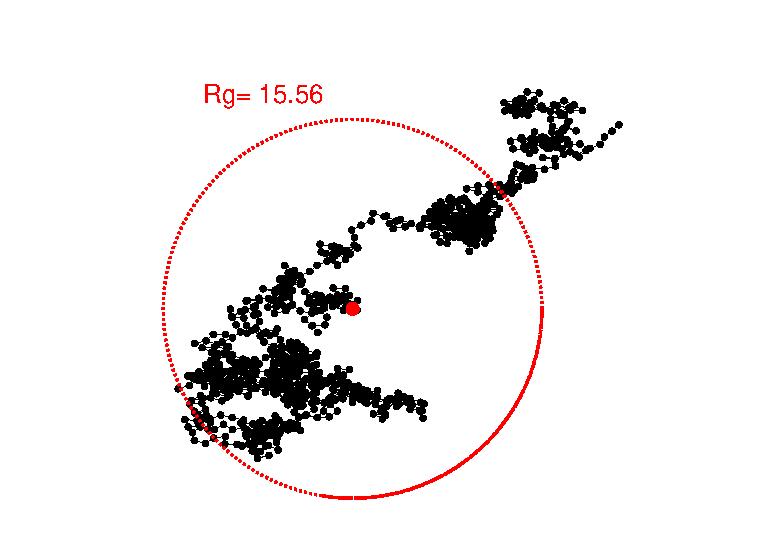
\includegraphics[width=10cm]{RF_Rg.eps}
	\caption{自由連結鎖の慣性半径}
	\label{fig: RF_Rg}
\end{figure}

実際の測定においては、高分子鎖の末端を見出すことは困難で特定の条件がそろわない限り
\footnote
{
高分子鎖の一端から逆の端まで双極子モーメントの向きがそろったようなポリマーを対象とした誘電測定により末端間距離を測定できる場合があるが、こういう系は特殊である。
}、末端間距離 $R$ を実測することは困難である。
一方、慣性半径 $R_g$ は光散乱測定により実測することが可能である。
したがって、必要に応じて、慣性半径 $R_g$ を測定して (\ref{eq:rg_r}) 式の関係を通して末端間距離 $R$ へと換算することが可能である。

\subsection{高分子鎖のモデル}

ここでは、仮想的なセグメントを用いて記述された自由連結鎖という抽象的なモデルと、実際の分子に近いモデルとの関連について、もう少しだけ考察しよう。

前述の自由連結鎖においては、ボンドの角度についての規制を全く考慮していなかった。
しかしながら、実際のポリマー鎖においては、二つの C-C 結合の間には結合角が存在する。
さらには、結合が連結していることにより、以前にニューマン投影式を用いて議論したようにその結合周りの回転も束縛を受けていることになる。

このような拘束条件を考慮したモデルとして、C-C 結合の結合角だけを考慮した「自由回転鎖」モデル、および、配座に応じた回転の束縛を考慮した「束縛回転鎖」モデルの二つがよく知られている。

自由回転鎖モデルでの平均二乗末端間距離 $R_{fr}^2$ は、以下のように表記される
\footnote
{
この導出については、\ref{sec:1FR_R2} を参照されたい。
}。
\begin{align}
R_{fr}^2 = Na^2 \dfrac{1+\cos \theta}{1-\cos \theta}
\label{eq:r2_sokubaku}
\end{align}

具体的な $\theta$ の値として、前述の $\theta = 180-109.5= 70.5^o$ を用いる
\footnote
{
ボンドベクトルの成す角であるので、C-C 結合の結合角 $109.5^o$ の外角となることに注意。
}と、$R_{fr}^2 \simeq 2 \times R^2$ となり、自由連結鎖の末端間距離の $\sqrt{2}$ 倍に増加することが判る。


一方、束縛回転鎖モデルでは、以下のように表すことができる(導出および詳細な議論は省略する)。
\begin{align}
R_{rr}^2 = Na^2 \dfrac{1+\cos \theta}{1-\cos \theta} \dfrac{1+ \langle \cos \theta \rangle}{1- \langle \cos \theta \rangle}
\label{eq:r2_sokubaku}
\end{align}
ここで、
\begin{align}
\langle \cos \theta \rangle = \dfrac{\displaystyle \int_0^{2 \pi} \cos \phi \exp [-u(\phi)/k_B T] d \phi}{\displaystyle \int_0^{2\pi} \exp [-u(\phi)/k_B T] d \phi}
\end{align}

(\ref{eq:r2_sokubaku}) 式に表れた $Na^2$ にかかる係数項($\cos \theta$ および $\langle \cos \theta \rangle$ に関する分数の因子)は、「束縛回転鎖」モデルにおいても、定数項として取り扱えるので、結局、
自由回転鎖モデルと同様に、末端間距離の増加という因子として働くことになる。

したがって、現実のポリマー鎖に近くなるように結合角を考慮した場合でも、末端間距離は、$N^{1/2}$ に比例する(比例定数は $> 1$ となっている)ことが確認できる。
なお、この比例定数に対応するものが、特性比 $C_{\infty}$ であり、このことについては後ほど議論する。

\subsection{ガウス鎖について}

ここまでに示したように、高分子の主鎖を形成するボンドは熱運動のために、非常に多くの配座(コンフォメーション)を取ることができるのであった(極低温は除く)。
このような状態を考慮した場合、末端間距離の平均は分子量の $1/2$ 乗に比例し、かつ、その分布 $P(\bm{R})$ は、ガウス分布
\footnote
{
ガウス分布については、\ref{sec:gauss} を参照していただきたい。
}に従うことを示すことができる(導出は省略)。
\begin{align}
P(\bm{R}) =\left( \dfrac{3}{2 \pi N b_0^2} \right)^{3/2} \exp \left[ -\dfrac{3|\bm{R}|^2}{2Nb_0^2} \right]
\end{align}

高分子鎖が十分に長いと考えた場合、その一部分だけを取り出した部分鎖の末端間距離もガウス分布に従うと考えることができるようになる。
このように、部分鎖と全体とを比べても、スケールフリーに同様なガウス性を有するポリマー鎖をガウス鎖と呼んでいる。

\subsection{章末問題}
	\begin{enumerate}
	\item
	\label{it:3-1}
	(ランダムなボンドベクトルの発生)\\
	単位長さのボンドベクトルを任意の方向にランダムに発生させるためには、どのように三角関数を使えばよいのでしょうか。\\
	(ヒント)\\
	単位長さが任意の方向にランダムに向いているということは、円を描くことに相当します。つまり、ランダムに半径軸を発生させて、その x および y 座標を使えばよいわけです。

	\item
	\label{it:3-2}
	(二乗平均の意味)\\
	なぜ、二乗平均のように面倒くさいことをやっているのでしょうか。\\
	(ヒント)\\
	ポリマー鎖を構成しているセグメントが自由に動くことを想像して、$\langle \bm{R} \rangle$ がどうなるかを考えてみてください。

	\item
	\label{it:3-3}
	(自由連結鎖のボンドベクトル)\\
	(\ref{eq:r2})式で、四行目から五行目へと展開できることを説明してください。。\\
	(ヒント)\\
	これも、セグメントが自由に動いた場合に、ボンドベクトルがどのようにふるまうかを考えてみてください。

	\end{enumerate}

\newpage
% \section{高分子の分子量}

% 高分子は多数のモノマーが連結したものであり、一つの分子が非常に大きな分子量を有していることになる。
% この分子量という「数」を明確に定義することで、「長さ」あるいは「エントロピー」のような物理量を導出でき、材料設計に役立つ情報とすることができる。

% 高分子を材料として使いこなしていくためには、使用条件下でどのぐらいの大きさを占めているのかを見積もることが必要になる場合が多い。
% 例えば、ミクロ相分離のような構造において界面近傍での挙動を記述する際には、ポリマー鎖の変形がどのように生じているのかを考察するためには、バルク状態での鎖の大きさを知る必要がある。
% また、高分子を希釈して使用する場合にも、それぞれのポリマー鎖がどの程度重なり合うのかに応じて巨視的な粘度等の挙動が大きく変化するので、希釈条件下での大きさの情報は重要である。
% 前章で示した慣性半径のような特徴長さは、分子量 $N$ に対して以下の関係があり、
% \begin{align*}
% \begin{cases}
% \text{高分子の大きさを表す長さ} \propto N^{1/2} \\[8pt]
% \text{高分子の体積} \propto N^{3/2}
% \end{cases}
% \end{align*}
% 高分子の大きさの変化の傾向を見積もることができるようになる。


% また、分子量の増加に伴い分子間あるいは分子内における相互作用点が多くなり、マクロな物性値は変化する。
% さらに、連結数(重合度)の増加とともに、それぞれの連結において取りうる配座の数は、指数関数的に増加する。
% このことは、統計力学的なエントロピーの増加に他ならない。

% したがって、材料としての機能を設計するためには、高分子の分子量を定義することは重要である。
% 以下に、高分子の大きさを見積もるために必要となる分子量の決定方法について、簡単に記述しよう。


% \subsection{分子量の表し方}

% 合成高分子は、その合成法によって規定される統計的偶然性のために、分子量の分布を生じてしまう。
% したがって、高分子の分子量は、低分子化合物とは異なり、分子量の平均すなわち平均分子量で表さざるを得ないことになる。
% その平均の仕方には、各種考えられるが、一般に以下の二つが多用されている。

% なお、ここでは、分子量が $M_i$ の高分子鎖が $n_i$ 本含まれている系(ただし、インデックス変数 $i$ は、 $i=0,1,\cdots$)を対象として考えている
% \footnote
% {
% ここで、用いている $i$ というインデックスは、系中に存在するすべてのポリマー鎖を一本ずつ調べてヒストグラムで表した場合に、ヒストグラム中の何番目の括りに入っているのかということを表している。
% }。


% このとき、$\dfrac{n_i}{\sum_i n_i}$ は、すべての分画の本数を足し合わせたもので $i$ 成分の本数を割ったものであるので、$i$ 成分の数分率を表し、また、$w_i=\dfrac{n_i M_i}{\sum_i n_i M_i}$ は、$i$ 成分の重量分率を表していることになる。

% \begin{itemize}
% \item
% 数平均分子量

% これは、以下の式で表されるように、数(分子の本数)平均で分子量を表したものであり、分子の個数を評価することにより決定できる(章末問題 \ref{it:4-1})。

% この表現の分子量は、例えば、末端基定量法や浸透圧法により測定できる。
% \begin{align}
% {\bar M}_n 
% 	&= \dfrac{\sum_i n_i M_i}{\sum_i n_i} \notag \\[6pt]
% %	= \dfrac{n_0 M_0}{\displaystyle \sum_i n_i} + \dfrac{n_1 M_1}{\displaystyle \sum_i n_i}
% 	&= \dfrac{1}{\sum_i \left(\dfrac{w_i}{M_i} \right)}
% \label{eq:Mn}
% \end{align}

% \item
% 重量平均分子量

% 任意のインデックス $i$ で指定されるポリマーの重量 $n_i M_i$ の重量分率で分子量を平均化したものであり、光散乱法や沈降平衡法により測定できる。

% これは、以下のような表式で表される(章末問題 \ref{it:4-2})。
% \begin{align}
% {\bar M}_w 
% 	&= \dfrac{\sum_i n_i M_i^2}{\sum_i n_i M_i}\notag \\[6pt]
% %	&= \dfrac{n_0 M_0^2}{\displaystyle \sum_i n_i M_i} + \dfrac{n_1 M_1^2}{\displaystyle \sum_i n_i M_i} + \cdots \notag \\[6pt]
% %	&= M_0 \dfrac{n_0 M_0}{\displaystyle \sum_i n_i M_i} + M_1 \dfrac{n_1 M_1}{\displaystyle \sum_i n_i M_i} + \cdots \notag \\[6pt]
% %	&= M_0 w_0 + M_1 w_1 + \cdots \notag \\[6pt]
% 	&= \displaystyle \sum_i w_i M_i
% \label{eq:Mw}
% \end{align}

% \end{itemize}

% ここまでは、ヒストグラムとして取り扱えるように、離散的(整数のようなとびとびの値)に分画した議論を行ってきた。

% 通常、我々が扱う高分子の分子量は非常に大きいものであるので、分子量 $M$ を連続的な量であるとみなしても問題ない。
% 任意の試料において、分子量 $M$ と $M+dM$ の間にある分子の数分率を$f_n(M)dM$、重量分率を$f_w(M)dM$ と置くと、$f_n(M)$ および $f_w(M)$ は、それぞれ、数微分分布関数および重量微分分布関数となる。
% このとき、数平均分子量 $M_n$、および、重量平均分子量 $M_w$ は、それぞれ、以下のように積分を用いた連続的な表現に書き直すことができる
% \footnote
% {
% 統計では、確率変数 $X$ の期待値(平均値)$E(x)$ は、確率密度関数 $f(x)$ を用いて、以下のように書くことができる。
% \begin{align*}
% E(x) = \displaystyle \int x f(x) dx
% \end{align*}
% }。
% \begin{align}
% \begin{cases}
% M_n = \displaystyle\int_0^{\infty} M f_n (M)dM \\[10pt]
% M_w = \displaystyle\int_0^{\infty} M f_w (M)dM
% \end{cases}
% % = \dfrac{1}{\displaystyle\int_0^{\infty} \dfrac{1}{M} f_w (M)dM}
% \end{align}

% \subsection{分子量分布}

% 前述のように、合成高分子は分子量の分布を生じてしまうのであった。
% その分布の度合いは、分布関数の標準偏差により評価することができる(章末問題 \ref{it:4-3})。

% 高分子鎖の本数に関する分布関数の標準偏差 $s_n$ は以下のように定義され
% \footnote
% {
% 一般に、標準偏差は、平均値 $\mu$ を用いて、以下のように定義されている。
% \begin{align*}
% s^2
% 	&= \displaystyle \int(x - \mu)^2 f(x) dx
% \end{align*}
% }、
% \begin{align}
% s_n^2
% 	&= \displaystyle \int_0^{\infty}(M - \bar{M_n})^2 f_n(M) dM
% \end{align}
% ここから、以下の式が導出できる
% \footnote
% {
% この導出過程は、\ref{sec:MwMn} に示した。
% }。
% \begin{align}
% \dfrac{s_n}{\bar{M}_n} = \left(\dfrac{\bar{M}_w}{\bar{M}_n}-1\right)^{1/2}
% \end{align}

% 標準偏差 $s_n$ が大きいということが分布関数の幅が広い、すなわち、不均一の度合いが大きいことを表しているのであった。
% 上式において、$\dfrac{\bar{M}_w}{\bar{M}_n}$ が 1 よりも大きいほど右辺が大きくなり、一方、左辺は $\bar{M}_n$ は定数であるので、分子量の不均一度が大きいことになる。
% これが、$\dfrac{\bar{M}_w}{\bar{M}_n}$ が分子量分布の幅を見積もる指標となる理由の説明である。
 
% GPC(Gel Permiation Chromatography)法は、多孔性の高分子ゲルからなるカラムに高分子溶液を流し、分子量の大きい順に溶出してきた高分子溶液の濃度を測定する方法である。
% 単分散高分子試料を用いて校正曲線を作成することで、試験試料中の分子量の異なるポリマーの重量分率の分布を決定することができる。
% 上述したように、重量分率 $w_i$ の分布関数が求まれば、数平均分子量 $\bar{M}_n$ および重量平均分子量 $\bar{M}_w$ を求められるのであったから、GPC法により、それぞれの平均分子量および分子量分布の不均一度が同時に測定できることになる。



% \subsection{章末問題}

% 	\begin{enumerate}
% 	\item
% 	(和のとり方の確認)\\
% 		\vspace{-5mm}
% 		\begin{enumerate}
% 		\item
% 		\label{it:4-1}
% 		(\ref{eq:Mn}) 式の二行目への展開を実際にやってみてください。\\
% 		(ヒント)\\
% 		$\sum$ で表現されている和を実際に開いてみて、$w_i$ とよく見比べてみてください。

% 		\item
% 		\label{it:4-2}
% 		(\ref{eq:Mw}) 式の二行目への展開を実際にやってみてください。\\
% 		(ヒント)\\
% 		上のクイズと同様に、$\sum$ で表現されている和を実際に開いてみてください。
% 		\end{enumerate}
% 	\item
% 	(分子量分布の指標)\\
% 	\label{it:4-3}
% 	$\dfrac{\bar{M}_w}{\bar{M}_n}$ が、分子量の広がりを評価する指標となる理由について、説明してください。

% 	\end{enumerate}

\newpage

\section{高分子鎖のモデルと実在鎖との関係}

\ref{sec:CG_model} 章で、実在の高分子鎖を大幅に簡略化した「自由連結鎖」、あるいは、ある程度結合状態を考慮した「自由回転鎖」および「束縛回転鎖」モデルを用いた末端間距離 $R$ および慣性半径 $R_g$ についての議論を行った。
ここでは、実際の測定により得られる慣性半径および分子量と上記モデルからの理論値とを繋げていく議論を進めよう。


\subsection{特性比 $C_{\infty}$}

任意のセグメント数 $n$ である場合の末端間距離の実測値と自由連結鎖モデルでの理論値とを、以下のように比較することを考えよう。
\begin{align}
C_n=\dfrac{ \langle R_n^2 \rangle }{n b^2}
\end{align}
なお、理想鎖として取り扱えるように $\theta$ 状態で末端間距離を実測し、ボンド長さ $b$ は C-C 結合の 1.54 \AA を用いる。

この値は、自由連結鎖と比較して実在鎖がどのぐらい膨らんでいるかを表しており、一般にセグメント数の増加に伴い増加し、やがて、一定値に収束することが確かめられている。
したがって、特性比 $C_{\infty}$ は、上記の値を分子量を無限大に外挿した形で、以下のように定義されている。
\begin{align}
C_{\infty}=\lim_{n \to \infty} C_n 
%= \dfrac{ \langle R_N^2 \rangle }{N b^2}=\lim_{N \to \infty} \dfrac{ 6 \langle R_g^2 \rangle }{N b^2}
\label{fig:CR}
\end{align}
しかしながら、実際に分子量を無限大にするわけではなく、ある程度以上大きな繰り返し数のポリマーの慣性半径を数点実測することにより一定に収束していることを確認すればよい。

これまでの議論では、仮想的なモデルとしてセグメントの数 $N$ を設定して議論を行ってきた。
ここに、実測の分子量から見積もった重合度 $DP$(Degree of Polymerization: ポリマーの分子量をモノマーの分子量で除した値であり、モノマーの繰り返し数)を使用することで、仮想的なモデルと実在鎖との相関を議論することができる。
なお、この時の分子量としては重量平均分子量 $M_w$ を用いることが妥当である。

\begin{align}
C_{\infty} = \lim_{DP \to \infty} \dfrac{ \text{二乗平均末端間距離の実測値} }{DP \times b^2}
\label{fig:CR}
\end{align}

慣性半径 $R_g$ は実測可能であるので、これを用いて上式中の二乗平均末端間距離の実測値を求めると、例えばポリエチレンで $C_{\infty} \simeq 6.7$ 程度の値となっている。
すなわち、自由連結モデルよりも実在鎖は 7 倍程度膨らんでいるわけであり、この原因はボンドの角度に束縛が入っているためと考えることができる。

例えば、束縛回転鎖モデルでは、(\ref{eq:r2_sokubaku}) 式の $\dfrac{1+\cos \theta}{1-\cos \theta} \dfrac{1+ \langle \cos \theta \rangle}{1- \langle \cos \theta \rangle}$ の因子が、$C_{\infty}$ に対応することになり、トランスとゴーシュの排除が入ることを考慮するとこの値は 4 程度と計算され、1,5 位の相互作用であるペンタン効果を考慮することで、ほぼ実測と近い結果が得られるようである。

また、この特性比は、高分子鎖に置換基が入ることで増加し、かさ高いフェニル基を有するポリスチレンでは、10 程度となっている。



\subsection{有効結合長}

ここまでの自由連結鎖の議論において用いてきたボンド(ボンド長さ $b$)を m 個まとめて、新たなボンドとしてボンド長が $a$ となるボンドベクトルを考えよう。
%このとき、
%\begin{align}
%{\bf a}_i = 
%\end{align}
図 \ref{fig: EBL} にそのイメージを示した。
黒矢印で描かれた元のボンド(ボンド長さ $b$)に対して、青色で示した新たなボンド(ボンド長が $a$)を末端間ベクトル(図中の赤矢印)が同一となるように定義することができる。
\begin{figure}[htb]
 \centering
	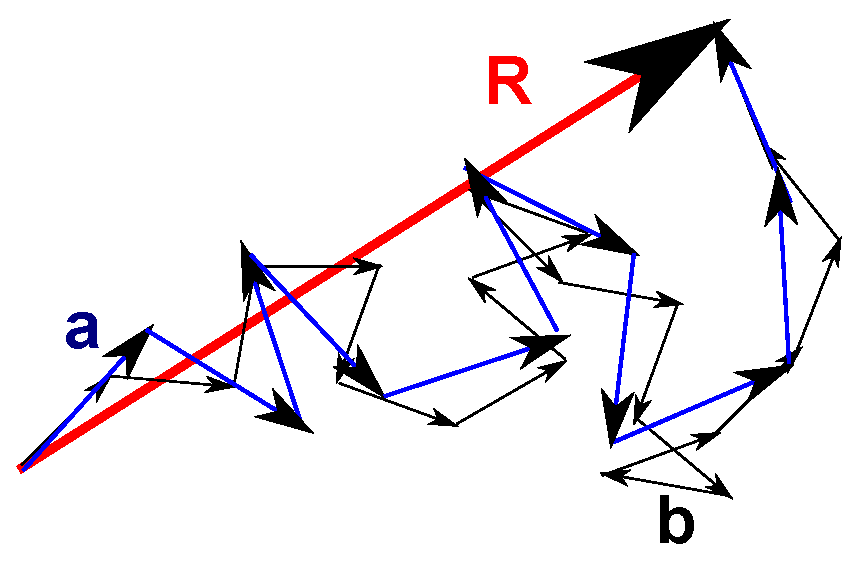
\includegraphics[width=6cm]{EBL.eps}
	\caption{有効結合長 a のイメージ}
	\label{fig: EBL}
\end{figure}

ここでは、末端間ボンドベクトル ${\bf R}$ が変化しないように同一の高分子鎖上に新たなボンドベクトル ${\bf a}$ を設定しているのであるから、新たなセグメント数 $N'=\dfrac{N}{m}$ を用いて、以下となる。
\begin{align}
&\langle R^2 \rangle = N b^2 = N' a^2 = \left(\dfrac{N}{m}\right) a^2 \notag \\
\therefore \quad &a = m^{1/2} b
\label{eq:EBL}
\end{align}

m は 1 以上の任意の数を設定することができ、このように設定した $a$ のことを有効結合長と呼ぶ。 
m の取り方によって、高分子鎖のそれぞれのボンド長さの総和、すなわち、$Nb$ で表される伸び切った鎖の長さは変化することになる。
これは、鎖に沿ったように見た場合の粗視化の度合いを表していることになり、m=N の極限では、伸び切り鎖長は末端間距離と等しいことになる。

図 \ref{fig: RF} に示した 1000 セグメントからなる自由連結鎖を、100 セグメントごとにまとめて 10 セグメントに粗視化し、元の 100 セグメントの重心を中心に有効結合長を直径とする円で表したものを図 \ref{fig: RF_CG} に示した。
\begin{figure}[htb]
 \centering
	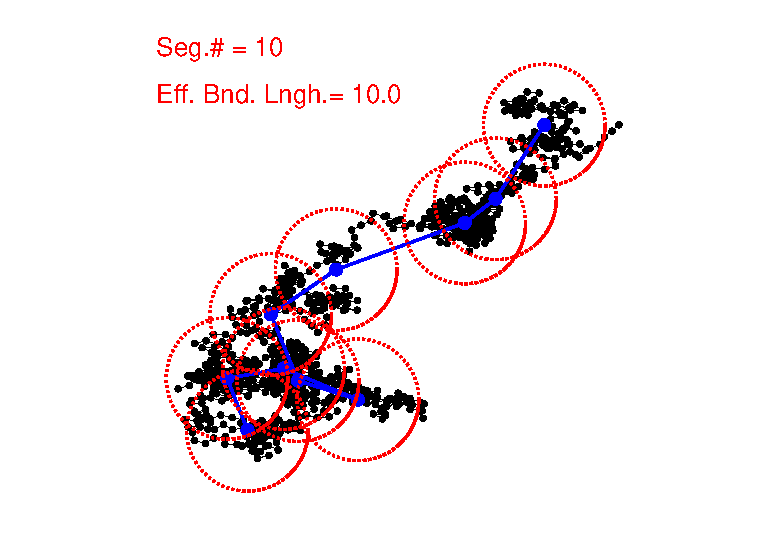
\includegraphics[width=10cm]{RF_CG.eps}
	\caption{粗視化セグメントのイメージ}
	\label{fig: RF_CG}
\end{figure}

これまでの議論では暗黙の裡に、新たなボンドベクトルが同一のボンド長を有するように記述してきたが、この設定は以下に示したような二種類のやり方を考えることができる
\begin{enumerate}
\item
結節点の位置を再現するように、それぞれのボンド長が異なる新たなボンドベクトル ${\bm a}_k$ を設定。
\begin{align*}
{\bm a}_k = \sum_{i=kN/m}^{kN/m + m-1} {\bm b}_i 
\end{align*}
\item
(\ref{eq:EBL}) 式で定義したボンド長 a となる新たなボンドベクトルを末端間ボンドベクトル ${\bf R}$ が変化しないように同一の高分子鎖上に設定する。
このとき、結節点の位置は再現できないことになる。
\end{enumerate}

このようなスケールのとり直しを、実測値により得られた (\ref{fig:CR}) 式の特性比を用いて行うと、
\begin{align}
\text{二乗平均末端間距離の実測値} &= C_{\infty} \times DP \times b^2 = DP \times a^2 \notag \\
\therefore \quad a &= C_{\infty}^{1/2} b
\end{align}
となり、実在の高分子鎖を有効結合長 a の自由連結鎖として表すことができるようになる。

\subsection{クーン長}

有効結合長という考え方を使った定義として、Kuhn が提案したクーン長($b_k$)がある。

これは、前節と同様に実在鎖に対して有効結合長を定義する際に、以下のように伸び切り鎖の長さが同一となるという境界条件を付与して、$N_k$ 個のセグメントに取り直すという定義である。
この定義の意味は、高分子鎖に沿ってみた場合の長さを変化させないという意味で、粗視化する際の最小限の単位長さを表していると考えることができる。
\begin{align}
 \begin{cases}
	C_{\infty} DP \times b^2 = N_k b_k^2 \\
	DP \times b = N_k b_k
 \end{cases}
\end{align}

具体的な値としては、この連立方程式を解いて、
\begin{align}
b_k = C_{\infty} b \notag \\
N_k = \dfrac{N}{C_{\infty} }
\end{align}
となる。

\newpage


\section{メゾ~マクロスケールでの高分子の特徴的なふるまい}

%\subsection{分子量と各種特性との関係}
%
%高分子が示す各種の特性には、粒子の数(ポリマー鎖の本数)への依存が弱いものと強いものとの二種類に大別すつことができる。
%
%逆説的に聞こえるかもしれないが、ポリマー鎖の本数によって決定できる物理量は、数への依存が弱いものと分類できる。
%
%
%例えば、浸透圧測定による数平均分子量の測定は、この原理に依ったものである。

\subsection{ゴム弾性}

高分子のゴム状態における弾性は、分子の広がり(配座の多様さ)に起因する{\bf エントロピー弾性}が支配的であるとされている。
このことの、熱力学的考察に基づく検討結果について、簡単に示す。

\subsubsection{熱力学的考察による検討}

ゴムの弾性的特徴を熱力学的立場から考察してみよう。

ゴムの試料に張力 $f$ をかけて、$x$ 軸方向に試料の長さが $L$ から微小量 $\odif{L}$ だけ伸長される{\bf 準静的過程}を考える。
このときの内部エネルギー $E$ に対する熱力学第 1 法則は、
\begin{align*}
	\odif{E} = T \odif{S} − p \odif{V} + f \odif{L}
\end{align*}
となり、ゴムの変形では体積が一定に保たれる(非圧縮性)ので、$\odif{V} = 0$ とおき、定圧定温条件下でこの式を $\odif{L}$ で割ると、
\begin{align*}
f = \left( \difp{E}{L} \right)_{p, T} -T\left( \difp{S}{L} \right)_{p, T}
\end{align*}
となる。

上式の第 1 項は内部エネルギーが原因となって生じる張力を、また、第 2 項はエントロピー変化が原因となって生じる張力を表していることになり、張力の起源によって二つの部分に分離して、それぞれを、エネルギー弾性、エントロピー弾性と呼ぶ。


\subsubsection{張力をエネルギー弾性とエントロピー弾性に分離する方法}

ここで 2 次微係数に対するマクスウェルの関係式より、
\begin{align*}
- \left( \difp{S}{L} \right)_{p, T} = \left( \difp{f}{T} \right)_{p, L}
\end{align*}
となり、この関係を用いると張力は、
\begin{align*}
f = \left( \difp{E}{L} \right)_{p, T} + T \left( \difp{f}{T} \right)_{p, L}
\end{align*}
となる。

ゴムにおいては、実際の伸長実験の温度依存性をこの式を用いて処理することにより、エントロピー弾性が支配的であることが「実験的に確認」されている。

%接線の傾き
%図 2.1 
%
%
%今,定圧下でゴムを伸長し,x 軸方向の長さ L を一定に保ちながら温度を変化させて張
%力を測定し,その結果を温度 T に対してプロットしたものとする(図 2.1).関係(2.4)
%によると,この曲線にある温度 T で接線を引き,それを絶対 0 度に外挿した値(C 点)を
%読みとると,その大きさが第 1 項のエネルギーによる部分を与えることがわかる.エント
%ロピー部分は全体からエネルギー部分を差し引いた AB の部分で与えられる.このように
%して張力を様々の温度で二つの部分に分離することが可能である.温度 20◦C での試料の
%長さ L0 を基準値として様々な伸長度 L/L0 に対してこの操作を行い,得た結果の例を図
%
%
%(曲線 B)とに分離した結果.ゴムの場合大部分がエントロピー弾性であることがわ
%かる.
%2.2 に示してある.この結果から,加硫ゴムの場合,その弾性の大部分がエントロピーに
%起因していることがわかる.

%さて,式(2.4)より,全張力のうちエネルギー張力が占める割合は
%fe
%f = 1 −
%! ∂ ln f
%∂ ln T
%"
%p,L
%= −T
%#
%∂ ln(f/T)
%∂T
%$
%p,L
%(2.5)
%となるが,右辺は張力の温度微係数とよばれる.以下の章で説明する分子論では,この温
%度微係数はネットワーク中の部分鎖の平均 2 乗末端間距離 < r2 >0 の温度変化と結びつ
%いていることが示され,
%fe
%f = T d ln < r2 >0
%dT (2.6)
%となる.左辺は熱力学量,右辺は鎖状分子に関する分子論的量なので,現象論的考察が分
%子論的視点から説明されたことになる.表 2.1 に T = 298 K での左辺の巨視的な測定値
%と右辺の分子論的な測定値の比較結果を示す.
%ポリエチレン(PE)で fe/f = −0.42 と負の数になるのは-CH2-CH2-CH2-鎖がトラ
%ンスのコンホメーションで伸びた状態になっているものが昇温によりゴーシュのコンホ
%メーションが増加し,末端間距離が減少するからである.また,ポリジメチルシロキサン
%(PDMS)で fe/f = 0.20 と大きな正の値になるのは-Si-O-Si-O-骨格がトランスのコンホ
%メーションではコンパクトな環状に丸まっているが,昇温によりゴーシュが増え,末端間
%距離が急増するからである.

\subsubsection{エントロピー弾性の直感的な理解}

前述のように、分子量の大きなポリマー鎖は、ガウス鎖とみなすことができる。
この両端のセグメントが外力によって自然長から伸長された場合、鎖がとりうる配位の数が少なくなりエントロピー $S$ が減少する。
この時、内部エネルギー $E$ が変化しない
\footnote
{
理想状態では内部エネルギーの変化はないものとみなすことが妥当となる。
このような仮定の妥当性は、理想気体が適切な条件下(希薄・高温な状態等)では実在気体をよく表現できていることを思い出せば納得がいくであろう。
}
のであれば、自由エネルギー($F=E-TS$)が高い状態となることが理解できる。
これは、ばねを伸長した時のポテンシャルエネルギーの増加と全く同等であり、それを元に戻そうとして張力が生じるわけである。

この現象をミクロな分子運動論で考えれば、高分子鎖の伸長でトランス配座が増えた場合に、熱搖動により元のゴーシュの比率に戻ろうとする際に、
末端間を内側に引きずり込むような張力が発生するものと理解することもできる。

\subsubsection{一次元自由連結鎖モデルでのゴム弾性}

自由連結鎖の一次元モデルのエントロピーは、末端間距離 $R$ の関数として以下のように表記することができる
\footnote
{
この導出は、\ref{ssec:1DRW_S} に示しているので、参照していただきたい。
}。
\begin{align*}
S(R)
	&= C -\dfrac{ k_B}{2Nb^2}R^2 \quad \text{(ただし、$C$ は鎖長 $N$ に依存する定数項)}
\end{align*}


ここで対象としている自由連結鎖モデルにおいては、内部エネルギー $E$ の寄与のない理想状態を考えているので、末端間距離が $R$ である場合の Helmholtz の自由エネルギー $F(R)$ は、上述のエントロピー $S(R)$ を用いて、以下のように導出される。
\begin{align*}
F 	&= E - TS(R) \\
	&= -TS(R) \\
	&= -k_B T \left( N\ln N - \dfrac{N}{2} \ln \dfrac{N^2}{4} - \dfrac{R^2}{2Nb^2} \right) 
\end{align*}

したがって、高分子鎖の末端間距離 $R$ を変化させた場合に、鎖に生じる張力 $f(R)$は、上記の自由エネルギー $F(R)$ を末端間距離 $R$ で微分した形で、
\begin{align*}
f(R) 	
&= \left(\dfrac{\partial F(R)}{\partial R} \right)_T \\
	&=\dfrac{\partial}{\partial R} \left[ -k_B T \left( N\ln N - \dfrac{N}{2} \ln \dfrac{N^2}{4} - \dfrac{R^2}{2Nb^2} \right) \right]\\
	&=- \dfrac{k_B T R}{Nb^2}
\end{align*}
となる。

この表式を見れば、高分子鎖のゴム弾性がその伸長長さ(末端間距離)に比例し、また、温度にも比例することが理解できる。


\subsection{相分離}

異なるモノマーからなる高分子が相溶しない場合が多いことはよく知られた事実である
\footnote{
例えば、重水素化ポリスチレンとポリスチレンのようなわずかな違いでも、分子量が大きい場合には相分離してしまう。
}
。
これは、低分子は水と油のように極端に分子の性質が異なる場合以外の組み合わせでは、多少の分子構造の違いであれば、一般に相溶しやすい事とは大きく異なるふるまいである。
この特性は、高分子の分子量が大きいため、高分子の混合に伴うエントロピー変化
\footnote
{
例えば、フローリー・ハギンス理論での格子モデルでは、高分子の重心の並進エントロピーの寄与だけを考えている。
}
の寄与が小さくなり、わずかな構造変化に起因したエンタルピー項が強く影響するためであると説明されている。

%せん断や伸長のようなマクロな外的変形を高分子材料に適応することにより、ミクロなスケールで高分子鎖が配向することがよく知られている。
%このような鎖の配向現象は、マクロな刺激によるミクロ構造の制御と捉えることができる。

また、高分子材料において、偏析と呼ばれる物質の局所的な偏りが生じることもある。
この偏析現象の主たる原因の一つが、壁の近傍では高分子鎖が自由な形を取ってエントロピー(形態エントロピーと呼ばれる)を獲得することができず枯渇するためであることが知られている。
その結果、高分子の不在を補うために、低分子成分が壁近傍に局在化するわけである。

\subsection{章末問題}

	\begin{enumerate}
	\item
	(高分子鎖のゴム弾性)\\
		\vspace{-5mm}
		\begin{enumerate}
		\item
		\label{it:5-1}
		高分子鎖において、エントロピー起因でゴム弾性が生じることを直感的に説明してください。

		\item
		\label{it:5-2}
		高分子鎖のゴム弾性が温度に比例することを説明してください。
。
		\end{enumerate}
	\item
	(相分離)\\
	\label{it:5-3}
	高分子同士の混合が困難である理由について説明してください。

	\end{enumerate}

\newpage

\section{章末問題の解答例}

\begin{itemize}
\item
{\bf 第一章}

	\begin{enumerate}
		\item
		(メゾスケール)\\
		メゾスケールのことについて、できるだけ自分の言葉で説明してみてください。\\
		{\bf(解答例)}\\
		メソあるいはメゾとは、「中間」という意味を表す接頭語である。
		したがって、メゾスケールという言葉の示す大きさは、有機化学で対象とする炭素結合の長さ程度の、たかだか 1 nm 程度の大きさのミクロなスケールと、
		我々が目に見えて実感できるような1 mm 程度以上の大きさ(マクロスケール)の間を指すことになり、長さの次元で $10^6$ にも及ぶスケール領域ということになる。

		材料の力学特性のような機能は、一般に、マクロスケールで発現するものであるので、マクロで機能を有する材料の設計を行う際には、
		化学的な感覚でナノスケールの大きさで設計することと、実際に評価しているマクロスケールとの間のメゾスケールが重要になる場合が多い。

		例えば、高分子の場合、その鎖としての構造の自由度が非常に高く、低分子には見られない特有の形状を取ることができる。
		また、各種の構造間の遷移に伴う活性化エネルギーが熱エネルギー程度($\simeq k_B T$)であり、構造変換が容易に起こる。
		このようなことから、高分子材料においては、マクロな機能性へのメゾスケール構造の寄与が非常に大きいことが知られている。

		\item
		(高分子の形)\\
		高分子の形について、立体配置(コンフィギュレーション)と立体配座(コンフォメーション)という言葉を意識して、説明してください。\\
		{\bf(解答例)}\\
		立体配置は、モノマー内、あるいは、モノマー間の共有結合の生成により規定される構造の様式であり、頭-尾結合、幾何異性体、立体規則性等のモノマー単位の構造から、
		高分子鎖の主鎖の分岐やデンドリマー、環状構造のような大きなスケールの構造も含まれている。
		構造の大きさに関わらず、共有結合を切断することなしには異なる構造へと遷移できないものであり、高分子の特性を決定する大きな要因である。

		一方、立体配座は、高分子鎖中の C-C 単結合周りの回転に基づくものであり、一般に、熱揺らぎ程度で容易に遷移してしまうという特徴があり、
		化学構造式としては書き表すことが困難で実感しにくい。
		しかしながら、高分子の膨大な内部自由度の原因であり、ソフトマターとしての特徴的な機能発現に大きく寄与している。


	\end{enumerate}

\item
{\bf 第二章}

	\begin{enumerate}
		\item
		(モノマー単位の大きさの見積もり)\\
		文中に示したポリエチレンの平面ジグザグ構造に基づく伸び切り構造の大きさの見積もりを、具体的に説明してください。\\
		(ヒント)\\
		C-C 結合の結合長が 1.54 \AA、三つの炭素が形成する C-C-C 結合が約 $109.5^o$ の結合角ということを考慮して、平面ジグザグ構造でのモノマー二つ分の絵を書いてみれば、
		ポリマー鎖の伸長方向とそれに垂直な方向との長さが見積れます。

		{\bf(解答例)}\\
		鎖の伸長方向を考慮した場合の、モノマー単位での長さ、および、幅は下図のように書くことができる。
		\begin{figure}[htb]
		\centering
		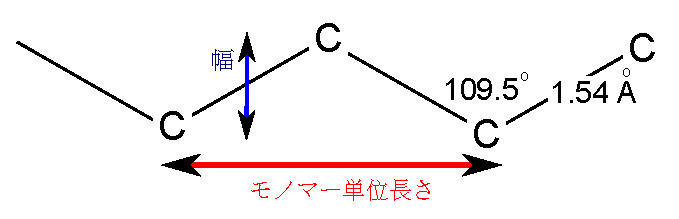
\includegraphics[width=6cm]{fig1.eps}
		\end{figure}

		このとき、伸び切り方向への長さは、
		\begin{align*}
		1.54 \times \cos (90 - 109.5/2) \times 2 \simeq 2.5 \text{\AA}
		\end{align*}
		また、幅は、
		\begin{align*}
		1.54 \times \sin (90 - 109.5/2) \simeq 0.9 \text{\AA}
		\end{align*}

		\item
		(伸び切り鎖の長さの見積もり)\\
		ポリエチレンの分子量が 10 万であった場合に、その平面ジグザグ構造の伸び切り鎖の長さが約 900 nm となることを、具体的に説明してください。\\
		(ヒント)\\
		分子量が 10 万であった場合に、その重合度がいくつであるかを算出すればいいだけです。

		{\bf(解答例)}\\
		ポリエチレンモノマーの分子量は、C$_2$H$_4 = 28$ であるから、ポリマーの分子量が 10 万ということは、100,000 $\div$ 28 $\simeq $3600 個のモノマーが
		重合していることになる。

		モノマーユニットの長さが 2.5 \AA であるので、鎖方向に伸長した場合には、$3600 \times 0.25 \simeq 900$ nm ということになる。

		\item
		(出現確率の比)\\
		エネルギーの異なる二つの状態(エネルギー差 $\Delta E$)の出現確率の比 $r(\Delta E)$ が以下の式となることを説明してください。
		\begin{equation*}
		r(\Delta E) = \exp(-\beta \Delta E)=\exp \left( -\dfrac{\Delta E}{k_B T} \right)
		\end{equation*}
		(ヒント)\\
		熱平衡状態であるカノニカル分布において、エネルギー準位が $E_i$ である状態 $i$ の出現確率 $P(E_i)$ は、下式で表されることを使って、
		二つのエネルギー状態の比を取ってください。\\
		なお、指数関数同士の割り算は、指数の引き算となります。
		\begin{align*}
		P(E_i) = \dfrac{1}{Z} \exp(-\beta E_i)
		\end{align*}

		{\bf(解答例)}\\
		低いほうのエネルギーを $E_l$ とし、高いほうを $E_h$ とした時、それぞれの状態の出現確率 $P(E_l), P(E_h)$ は、以下と書ける。
		\begin{align*}
			\begin{cases}
			P(E_l) = \dfrac{1}{Z} \exp(-\beta E_l) \notag \\[6pt]
			P(E_h) = \dfrac{1}{Z} \exp(-\beta E_h)
			\end{cases}
		\end{align*}

		このとき、$r(\Delta E)$ は、
		\begin{align*}
		r(\Delta E)
			&= \dfrac{P(E_h)}{P(E_l)} \notag \\[6pt]
			&=\dfrac{\left[ \dfrac{1}{Z} \exp(-\beta E_h) \right] }{\left[ \dfrac{1}{Z} \exp(-\beta E_l) \right]} \notag \\[6pt]
			&=\dfrac{\exp(-\beta E_h) }{\exp(-\beta E_l)} \notag \\[6pt]
			&=\exp(-\beta E_h - \{-\beta E_l \}) \notag \\[6pt]
			&=\exp(-\beta \{E_h - E_l \}) \notag \\[6pt]
			&=\exp(-\beta \Delta E)
		\end{align*}
		と書くことができる。\\
		(補足事項)\\
		ここに示したような二準位系において、それぞれのエネルギー準位に属する微視的状態の数が複数あった(縮退している)場合を考える。
		例えば、低いほうの準位の微視的状態の数 $W(E_l) = n_l$ で、高いほうを $W(E_h) = n_h$ とすると、上式は、
		\begin{align*}
		r(\Delta E)
			&= \dfrac{P(E_h)}{P(E_l)} \notag \\[6pt]
			&=\dfrac{\left[ \dfrac{1}{Z} W(E_h) \exp(-\beta E_h) \right] }{\left[ \dfrac{1}{Z} W(E_l) \exp(-\beta E_l) \right]} \notag \\[6pt]
			&=\dfrac{n_h \exp(-\beta E_h) }{n_l \exp(-\beta E_l)} \notag \\[6pt]
			&=\dfrac{n_h}{n_l} \dfrac{\exp(-\beta E_h) }{\exp(-\beta E_l)} \notag \\[6pt]
%			&=\dfrac{n_h}{n_l} \exp(-\beta E_h - \{-\beta E_l \}) \notag \\[6pt]
%			&=\dfrac{n_h}{n_l} \exp(-\beta \{E_h - E_l \}) \notag \\[6pt]
			&=\dfrac{n_h}{n_l} \exp(-\beta \Delta E)
		\end{align*}
		となり、縮退の数の因子が前に括りだされることになる。

		\item
		(鎖の曲り方の具体例)\\
		以下の二つのクイズを考えてください。

		\begin{enumerate}
			\item
			(ポリエチレンの例)\\
			室温($27^o$C)のポリエチレンで、トランスとゴーシュとのポテンシャル・エネルギー差 $\Delta \varepsilon$ が 2.1 kJ mol$^{-1}$ であったとした場合、
			トランス連鎖はどのぐらい続くと見積もればいいことになるでしょうか。\\
			(ヒント)\\
			(\ref{eq:ratio})式に、上記のエネルギー差を入れれば、それぞれの状態の出現確率の比が求まります。
			ただし、ゴーシュ状態のエネルギーは二つの微視的状態が縮退したものであることに注意してください。
			なお、$k_B \simeq 1.4 \times 10^{-23} {\rm J K}^{-1}$ です。 

			{\bf(解答例)}\\
			高いエネルギー準位であるゴーシュ状態は二つの微視的状態が縮退しているので、これを考慮して、
			\begin{align*}
			r(\Delta \varepsilon)
			&=\dfrac{2}{1}\exp \left( -\dfrac{\Delta \varepsilon}{k_B T} \right) \notag \\[6pt]
			&=2\exp \left( -\dfrac{-2.1 \times 10^3 {\rm J mol}^{-1} }{1.4 \times 10^{-23} {\rm J K}^{-1} \times 6.02 \times 10^{23} \times 300 {\rm K} } \right) 
			\notag \\[6pt] 
			&=2\exp \left( 0.83 \right)\notag \\[6pt]
			&\simeq4.6
			\end{align*}

			したがって、トランス連鎖としては、4.6 個程度と考えることができます。
			\item
			(持続長)\\
			このメモでは詳細に立ち入りませんが、高分子鎖の曲がりやすさを考慮したモデルとして、ミミズ鎖(Worm-like chain)と呼ばれるものがあります。
			このモデルにおいては、粗視化した単位として、モノマー単位が平面ジグザグ構造でまっすぐにつながる長さを統計的に見積もって、
			「持続長 $l_p$」と呼ぶものを使います。\\
			持続長は、以下の表式で表されます。
			\begin{equation*}
			l_p = l_0 \exp \left( - \dfrac{\Delta \varepsilon}{k_B T} \right)
			\end{equation*}
			ここで、$l_0$ はモノマー単位の長さであり、ポリエチレンの場合は、C-C 結合の結合長 1.54 \AA を用います。\\
			この式を用いて、上記のポリエチレンの場合の持続長を求めてください。\\
			(ヒント)\\
			結局、統計的に見てトランス連鎖が続く状態を考えて、その具体的な長さを見ているだけです。

			{\bf(解答例)}\\
			与式に、代入して、
			\begin{align*}
			l_p 
			&= l_0 \exp \left( - \dfrac{\Delta \varepsilon}{k_B T} \right) \notag \\
			&\simeq 1.54 \times 4,6 \notag \\
			&= 7.1
			\end{align*}

			したがって、7 \AA 程度であることになる。	
		\end{enumerate}
	\item
	(トランス・ゴーシュの遷移)\\
	ブタンにおける C-C 結合周りの回転振動数は、$10^{12}$ sec$^{-1}$ のオーダーで生じるとして、トランス $\leftrightarrow$ ゴーシュの相互遷移のエネルギー障壁が、
	15 kJ mol$^{-1}$ 程度であるとした場合、室温での遷移の頻度を見積もってください。

	{\bf(解答例)}\\
	活性化エネルギーに対応するエネルギー障壁を乗り越えて状態が遷移していく過程の頻度は、
	系中に存在する粒子の中でその障壁に対応するエネルギーを持っている粒子の存在比率を考えればよいことになる。

	本設問の場合は、基本的な回転振動数(時間の逆数)が与えられているのであるから、系が注目する状態から他の状態(今回の場合は、トランス状態からゴーシュ状態)に遷移する
	緩和時間 $\tau$ の逆数の形で書き下すことができる。
		\begin{align*}
			\dfrac{1}{\tau}
			&= 10^{12} \times \exp \left( -\dfrac{\Delta E}{k_B T} \right) \notag \\[6pt]
			&= 10^{12} \times \exp \left( -\dfrac{15 \times 10^3 {\rm J mol}^{-1} }{1.4 \times 10^{-23} {\rm J K}^{-1} \times 6.02 \times 10^{23} 
			\times 300 {\rm K} } \right) \notag \\[6pt] 
			&\simeq 10^{12} \times \exp \left( -6 \right)\notag \\[6pt]
			&= 10^{12} \times 2.5 \times 10^{-3}\notag \\[6pt]
			&\simeq 10^{9}
			\end{align*}

	したがって、オーダーでみれば、三桁程度頻度が低下するという結論を得ることができる。

	\end{enumerate}

\item
{\bf 第三章}

	\begin{enumerate}
	\item
	\label{it:3-1}
	(ランダムなボンドベクトルの発生)\\
	単位長さのボンドベクトルを任意の方向にランダムに発生させるためには、どのように三角関数を使えばよいのでしょうか。\\
	(ヒント)\\
	単位長さが任意の方向にランダムに向いているということは、円を描くことに相当します。つまり、ランダムに半径軸を発生させて、
	その x および y 座標を使えばよいわけです。\\
	{\bf(解答例)}\\
	$xy$ 平面に、半径 $r$ の円を想定すれば、原点から円上の任意の点に向けたベクトルの $x$ 成分および $y$ 成分は、以下のように、$x = r \cos \theta$ 
	および $y= r \sin \theta$ で表されることになる。
		\begin{figure}[htb]
		\centering
		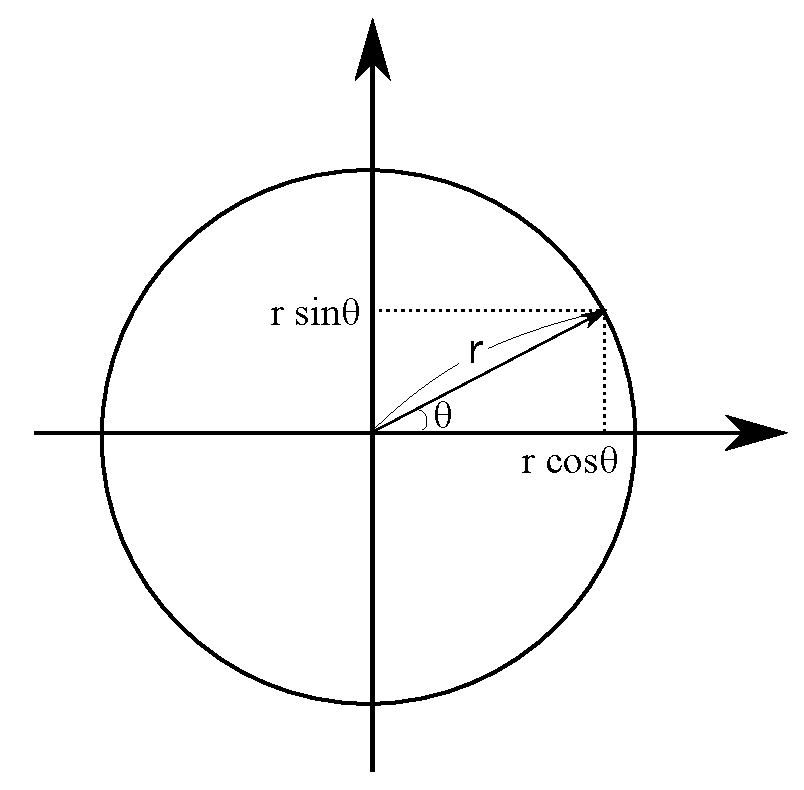
\includegraphics[width=5cm]{sin_cos.eps}
		\end{figure}

	したがって、任意の点 $(x,y)$ を始点とする任意の方向に向いたランダムな単位ベクトル(長さが常に 1 )は、$0 \sim 2\pi$ の範囲でランダムに中心角 $\theta$ を
	発生させて、終点を $(x+\cos \theta, y+\sin \theta)$ とすればよいことになる。


	\item
	(二乗平均の意味)\\
	なぜ、二乗平均のように面倒くさいことをやっているのでしょうか。\\
	(ヒント)\\
	ポリマー鎖を構成しているセグメントが自由に動くことを想像して、$\langle \bm{R} \rangle$ がどうなるかを考えてみてください。\\
	{\bf(解答例)}\\
	「セグメントを自由に配置させることができる」ということの意味を考えよう。
	ここでは、簡単のために、数直線上にセグメントを配置する一次元のモデルを考えよう。
	なお、ここでの議論は容易に三次元に拡張できる。

	一つのセグメントを原点に固定した場合、次のセグメントは、正の方向に配置されるとしても、また、逆に、負の方向に配置されるとしても、その生じる確率は等価となる。
	ということは、この二つのセグメントを結ぶボンドベクトルの平均(期待値)は、0 となるわけである。

	高分子鎖の末端間ベクトルというのは、片末端のセグメントからスタートして、逆側の末端のセグメントに至るボンドベクトルを一筆書きでつないだものと考えることができる。
	ここで、片方の末端にあるセグメントを原点にピン止めした場合を考えよう。
	複数のセグメントを配置するという多数のステップを進んだ場合でも、それぞれのボンドベクトルの期待値が 0 である。
	結局、高分子鎖の末端間ベクトルは ${\bm 0}$ となってしまう。

	しかしながら、二乗平均を取ることで、同一のボンドベクトルの二次の項が現れることになり、これは、ボンドベクトル長さの二乗の値を持つ。
	したがって、その末端からの距離を正の値として足し合わせることができ、末端間距離の二乗の平均を正の値として定義できることになる。

	\item
	(自由連結鎖のボンドベクトル)\\
	(\ref{eq:r2})式で、四行目から五行目へと展開できることを説明してください。。\\
	(ヒント)\\
	これも、セグメントが自由に動いた場合に、ボンドベクトルがどのようにふるまうかを考えてみてください。

	{\bf(解答例)}\\
	二乗平均を取るということを、具体的に表式として示そう。

	下式に示したように、まず、末端間ベクトルの二乗 $R^2$ は、以下のように各ボンドベクトル ${\bm u_i}$の和の形に書き下すことができる。
	\begin{align*}
	R^2
	&= \langle |\bm{R}|^2 \rangle \notag \\
	&=\langle |\bm{r}_0 - \bm{r}_N|^2 \rangle \notag \\
	&=\langle |(\bm{r}_1 - \bm{r}_0) + (\bm{r}_2 - \bm{r}_1) + \cdots + (\bm{r}_N - \bm{r}_{N-1})|^2 \rangle \notag \\
	&=\left\langle \left|\sum_{i=0}^{N-1}\bm{u}_i \right|^2 \right\rangle
	\end{align*}

	このとき、三行目のボンドベクトルの二乗平均は、以下のように、それ自身のボンドベクトルの二乗と他のボンドベクトルとの内積の形を用いて書きなおすことができる。
	\begin{align*}
	\left\langle \left|\sum_{i=0}^{N-1}\bm{u}_i \right|^2 \right\rangle
		&= \left\langle \left|\bm{u}_0 + \bm{u}_1 + \cdots \right| \cdot \left|\bm{u}_0 + \bm{u}_1 + \cdots \right| \right\rangle \notag \\
		&= \left[ \langle |\bm{u}_0|^2 \rangle + \langle|\bm{u}_1 |^2\rangle + \cdots \right] \notag \\
		&\quad +\left[ \langle \bm{u}_0 \cdot\bm{u}_1 \rangle + \langle \bm{u}_0 \cdot\bm{u}_2 \rangle + \cdots \right] \notag \\
		&\quad +\left[ \langle \bm{u}_1 \cdot\bm{u}_0 \rangle + \langle \bm{u}_1 \cdot\bm{u}_2 \rangle + \cdots \right] \notag \\
		&\quad + \cdots \notag \\
		&=\sum_{i=0}^{N-1} \left\langle \left|\bm{u}_i \right|^2 \right\rangle 
		+\sum_{i \neq j} \left\langle \bm{u}_i \cdot \bm{u}_j \right\rangle
	\end{align*}
	ここで、自由連結鎖におけるボンドベクトルの性質を確認しよう。
	それぞれのボンドベクトルは、方向について独立(無相関)であるから、
	\begin{align*}
	\langle \bm{u}_i \cdot \bm{u}_j \rangle 
	&= \langle \bm{\hat{u}}_i \cdot \bm{\hat{u}}_j \rangle a^2 \\
	&=
		\begin{cases}
		\langle |\bm{\hat{u}}_i |^2 \rangle a^2 = a^2	&\quad (\text{$i = j$ のとき}) \\
		\langle \bm{u}_i \rangle \cdot \langle \bm{u}_j \rangle = \bm{0}\cdot\bm{0} = 0	&\quad(\text{$i \neq j$ のとき})
		\end{cases}
	\end{align*}
	ここで、$\bm{\hat{u}}_i \equiv \dfrac{\bm{u}_i}{|\bm{u}_i|}$ は $\bm{u}_i$ 方向の単位ベクトル、$a$ はボンドの長さを表している。

	したがって、上記の自由連結鎖におけるボンドベクトルの性質を使って、
	\begin{align*}
	R^2
	&=\sum_{i=0}^{N-1} \left\langle \left|\bm{u}_i \right|^2 \right\rangle 
	+\sum_{i \neq j} \left\langle \bm{u}_i \cdot \bm{u}_j \right\rangle \notag \\
	&=\sum_{i=0}^{N-1} a^2 + \sum_{i \neq j} 0 \notag \\
	&= N a^2
	\end{align*}
	\end{enumerate}

\item
{\bf 第四章}
	\begin{enumerate}
	\item
	(和のとり方の確認)\\
		\vspace{-5mm}
		\begin{enumerate}
		\item
		(\ref{eq:Mn}) 式の二行目への展開を実際にやってみてください。\\
		(ヒント)\\
		$\sum$ で表現されている和を実際に開いてみて、$w_i$ とよく見比べてみてください。

		{\bf(解答例)}\\
		$\sum$ で表現されている和を実際に開いていこう。

		まず、逆数を取ったうえで、和を開いていく。
		\begin{align*}
		{\bar M}_n 
			&= \dfrac{\sum_i n_i M_i}{\sum_i n_i} \notag \\
			&= \dfrac{1}{\left( \dfrac{\sum_i n_i}{\sum_i n_i M_i} \right)} \notag \\
			&= \dfrac{1}{\left(\dfrac{n_0 + n_1 + \cdots}{\sum_i n_i M_i} \right)} \notag \\
			&= \dfrac{1}{\left(\dfrac{n_0 }{\sum_i n_i M_i} + \dfrac{n_1}{\sum_i n_i M_i} + \cdots \right)} \notag \\
			&= \dfrac{1}{\left(\dfrac{n_0 M_0}{M_0 \sum_i n_i M_i} + \dfrac{n_1 M_1}{M_1\sum_i n_i M_i} + \cdots \right)}
		\end{align*}
		三行目で分子の和を開いた後に、五行目では分子と分母に $M_i$ を掛けている。

		ここで、$w_i =\dfrac{n_i M_i}{\sum_i n_i M_i}$ と見比べると、分母の各因子が $\dfrac{w_i}{M_i}$ となっていることが分かる。

		したがって、以下のように展開を進めることができる。
		\begin{align*}
		{\bar M}_n 
			&= \dfrac{1}{\left(\dfrac{n_0 M_0}{M_0 \sum_i n_i M_i} + \dfrac{n_1 M_1}{M_1\sum_i n_i M_i} + \cdots \right)} \notag \\
			&= \dfrac{1}{\left(\dfrac{w_0}{M_0} + \dfrac{w_1}{M_1} + \cdots \right)} \notag \\
			&= \dfrac{1}{\sum_i \left(\dfrac{w_i}{M_i} \right)}
		\end{align*}

		\item
		(\ref{eq:Mw}) 式の二行目への展開を実際にやってみてください。\\
		(ヒント)\\
		上のクイズと同様に、$\sum$ で表現されている和を実際に開いてみてください。\\
		{\bf(解答例)}\\
		$\sum$ で表現されている和を実際に開くと、
		\begin{align*}
		{\bar M}_w 
			&= \dfrac{\sum_i n_i M_i^2}{\sum_i n_i M_i}\notag \\[6pt]
			&= \dfrac{n_0 M_0^2}{\displaystyle \sum_i n_i M_i} + \dfrac{n_1 M_1^2}{\displaystyle \sum_i n_i M_i} + \cdots \notag \\[6pt]
			&= M_0 \dfrac{n_0 M_0}{\displaystyle \sum_i n_i M_i} + M_1 \dfrac{n_1 M_1}{\displaystyle \sum_i n_i M_i} + \cdots \notag \\[6pt]
			&= M_0 w_0 + M_1 w_1 + \cdots \notag \\[6pt]
			&= \displaystyle \sum_i w_i M_i
		\end{align*}
		\end{enumerate}
	\item
	(分子量分布の指標)\\
	$\dfrac{\bar{M}_w}{\bar{M}_n}$ が、分子量の広がりを評価する指標となる理由について、説明してください。\\
	{\bf(解答例)}\\
	任意の分布関数があった場合、その分布の広がり方の度合いは、分布関数の標準偏差により評価することができる。

	高分子鎖の本数に関する分布関数(数平均分子量に対応)の標準偏差 $s_n$ は以下のように定義される。
	\begin{align}
	s_n^2
		&= \displaystyle \int_0^{\infty}(M - \bar{M_n})^2 f_n(M) dM
	\end{align}

	これは、以下のように展開することができる。
	\begin{align}
	s_n^2
		&= \displaystyle \int_0^{\infty}(M - \bar{M}_n)^2 f_n(M) dM \notag \\
		&= \displaystyle \int_0^{\infty}(M^2 - 2M \bar{M_n} + \bar{M}_n^2) f_n(M) dM \notag \\
		&= \displaystyle \int_0^{\infty} M^2 f_n(M) dM - 2 \bar{M}_n \displaystyle \int_0^{\infty} M f_n(M) dM + \bar{M}_n^2 \displaystyle \int_0^{\infty} 
			f_n(M) dM \notag \\
		&= \displaystyle \int_0^{\infty} M^2 f_n(M) dM - 2 \bar{M}_n \bar{M}_n + \bar{M}_n^2  \notag \\
		&= \displaystyle \int_0^{\infty} M^2 f_n(M) dM - \bar{M}_n^2
	\end{align}

	なお、四行目への展開においては、$\displaystyle \int_0^{\infty} M f_n(M) dM = \bar{M}_n$ と $\displaystyle \int_0^{\infty} f_n(M) dM = 1$ を用いた。

	ここで、(\ref{eq:Mw}) 式より、
	\begin{align}
	{\bar M}_w 
		&= \dfrac{\sum_i n_i M_i^2}{\sum_i n_i M_i}\notag \\[6pt]
		&= \dfrac{\sum_i n_i M_i^2}{\sum_i n_i} \times \dfrac{\sum_i n_i}{\sum_i n_i M_i}\notag \\[6pt]
		&= \displaystyle \int_0^{\infty} M^2 f_n(M) dM \times \dfrac{1}{\bar{M}_n }\notag \\[6pt]
	\therefore \displaystyle \int_0^{\infty} M^2 f_n(M) dM &= \bar{M}_n \bar{M}_w
	\end{align}
	なお、三行目への展開では、数微分分布関数 $f_n(M)$ の二次のモーメントであることを用いている。

	この結果を代入して、
	\begin{align}
	s_n^2 &= \bar{M}_n \bar{M}_w - \bar{M}_n^2\notag \\[6pt]
	\therefore \dfrac{s_n}{\bar{M}_n} &= \left(\dfrac{\bar{M}_w}{ \bar{M}_n} - 1 \right)^{-1/2}
	\end{align}
	を得る。
	なお、二行目へは、両辺を $\bar{M}_n^2$ で除した後に、平方根を取っている。

	標準偏差 $s_n$ が大きいということが分布関数の幅が広い、すなわち、不均一の度合いが大きいことを表しているのであった。

	上式において、$\dfrac{\bar{M}_w}{\bar{M}_n}$ が 1 よりも大きいほど右辺が大きくなり、一方、左辺は $\bar{M}_n$ は定数であるので、分子量の不均一度が大きいことになる。

	これが、$\dfrac{\bar{M}_w}{\bar{M}_n}$ が分子量分布の幅を見積もる指標となる理由の説明である。

	\end{enumerate}

\item
{\bf 第六章}
	\begin{enumerate}
	\item
	(高分子鎖のゴム弾性)\\
		\vspace{-5mm}
		\begin{enumerate}
		\item
		\label{it:5-1}
		高分子鎖において、エントロピー起因でゴム弾性が生じることを直感的に説明してください。\\
		{\bf(解答例)}\\
		(直感的な説明)

		分子量の大きなポリマー鎖は、ガウス鎖とみなすことができる。
		この両端のセグメントが外力によって自然長から伸長された場合、鎖がとりうる配位の数が少なくなりエントロピー $S$ が減少する。
		この時、内部エネルギー $E$ が変化しないと考えれば、自由エネルギー($F=E-TS$)が高い状態となることが理解できる。
		これは、ばねを伸長した時のポテンシャルエネルギーの増加と全く同等であり、それを元に戻そうとして張力が生じるわけである。

		\item
		\label{it:5-2}
		高分子鎖のゴム弾性が温度に比例することを説明してください。\\
		{\bf(解答例)}\\
		自由連結鎖の一次元モデルのエントロピーは、末端間距離 $R$ の関数として以下のように表記することができる。
		\begin{align*}
		S(R)
			&= C -\dfrac{ k_B}{2Nb^2}R^2 \quad \text{(ただし、$C$ は鎖長 $N$ に依存する定数項)}
		\end{align*}

		ここで対象としている自由連結鎖モデルにおいては、内部エネルギー $E$ の寄与のない理想状態を考えているので、末端間距離が $R$ である場合の 
		Helmholtz の自由エネルギー 	$F(R)$ は、上述のエントロピー $S(R)$ を用いて、以下のように導出される。
		\begin{align*}
		F 	&= E - TS(R) \\
			&= -TS(R) \\
			&= -k_B T \left( N\ln N - \dfrac{N}{2} \ln \dfrac{N^2}{4} - \dfrac{R^2}{2Nb^2} \right) 
		\end{align*}

		したがって、高分子鎖の末端間距離 $R$ を変化させた場合に、鎖に生じる張力 $f(R)$は、上記の自由エネルギー $F(R)$ を末端間距離 $R$ で微分した形で、
		\begin{align*}
		f(R) 	
		&= \left(\dfrac{\partial F(R)}{\partial R} \right)_T \\
			&=\dfrac{\partial}{\partial R} \left[ -k_B T \left( N\ln N - \dfrac{N}{2} \ln \dfrac{N^2}{4} - \dfrac{R^2}{2Nb^2} \right) \right]\\
			&=- \dfrac{k_B T R}{Nb^2}
		\end{align*}
		となる。

		上記の表式を見れば、高分子鎖のゴム弾性がその伸長長さ(末端間距離)に比例し、また、温度にも比例することが理解できる。

		\end{enumerate}
	\item
	(相分離)\\
	\label{it:5-3}
	高分子同士の混合が困難である理由について説明してください。\\
	{\bf(解答例)}\\
	物質を混合した場合、一様に混合するか、あるいは、二つの相に分離してしまうのかは、混合後の自由エネルギー(体積一定の系であれば以下のヘルムホルツ自由エネルギー)
	を評価することで判断できる。
	\begin{align*}
	F=E-TS
	\end{align*}

	低分子の場合では、多少異なる化合物であっても一様に混合する場合が多い。
	この事実は、異なる物質が混合した場合に生じる内部エネルギー($E$ の項)の増加と、混合前後での並進エントロピー増加によるエネルギー低下
	($-TS$ の項は$S$ の増加により減少する)を比べた場合、後者の寄与が大きいために混合に伴う自由エネルギー変化が負となり、
	一様混合状態が安定になるためと説明されている。

	一方、異なるモノマーからなる高分子が相溶しない場合が多いことはよく知られている。
	これは、高分子の分子量が大きいため、高分子の混合に伴うエントロピー変化が重合度の逆数の形で小さくなり、わずかな構造変化に起因した内部エネルギー項が
	強く影響するためであると説明されている。


	\end{enumerate}

\end{itemize}



\newpage
\begin{center}
{\Large \textgt{参考資料}}
\end{center}

以下の青字部分はリンクがついていますので、クリックしてください。

\begin{itemize}
\item
\href{http://www.kyoritsu-pub.co.jp/bookdetail/9784320043800}{「高分子化学 第5版」、共立出版、村橋 俊介・小高 忠男・蒲池 幹治・則末 尚志 編}

阪大の先生が書いた、一般的な高分子の教科書の一つです。

第一章「高分子科学序論」に目を通せばいいと思います。
余力があれば、第六章が役に立ちます。

\item
\href{http://www.kyoritsu-pub.co.jp/bookdetail/9784320043015}{「高分子の分子量」、共立出版、高分子学会 編集・五十野 善信他著}

絶版。ISBN	978-4-320-04301-5

このメモを書く際に、参考にしました。

\item
\href{https://dl.dropboxusercontent.com/u/18899343/Probability/Kitaiti_Bunsan/EV_Var.pdf}{「期待値と分散」}

統計的な処理を行う際に最も基本的な期待値(平均)と分散について、基礎的な事項を簡単にまとめた資料です。

\item
\href{https://dl.dropboxusercontent.com/u/18899343/Probability/Prob_Dist/Prob_Dist.pdf}{「確率分布関数」}

統計的な処理に必要となる分布関数についてまとめた資料です。


\item
\href{https://dl.dropboxusercontent.com/u/18899343/Thermo_Dynamics/basics/Thermo_Dynamics_basics.pdf}{「熱力学の基礎的事項」}

ここでの議論に必要となる、熱力学の基本的な事項をまとめたものです。
一応、演習問題がついています。

\item
\href{https://dl.dropboxusercontent.com/u/18899343/physics/FreeEnergyForm/Free_Energy_Form.pdf}{「混合系の相分離条件」}

高分子に限定することなく、一般的な相分離についてまとめたものです。

%\item
%\href{https://dl.dropboxusercontent.com/u/18899343/physics/FH_model/FH_model_2.pdf}{「フローリー・ハギンス格子モデルによる混合の自由エネルギー」}
%
%フローリー・ハギンス格子モデルに基づく、高分子を混合した際の自由エネルギー変化について、まとめたものです。
%
%\item
%\href{https://dl.dropboxusercontent.com/u/18899343/physics/Phase_Separation/Phase_Separation.pdf}{「ポリマーブレンドの相図」}
%
%ポリマーブレンドの相分離挙動についてまとめたものです。
%
%\item
%\href{https://dl.dropboxusercontent.com/u/18899343/physics/Miscibility_Window/Miscibility_Window.pdf}{「ランダム共重合体によるMiscibility Window について」}
%
%ランダム共重合体に特有の相溶性の窓といわれる事象について、まとめたものです。

%\item
%\href{https://dl.dropboxusercontent.com/u/18899343/physics/FreeEnergyForm/Free_Energy_Form.pdf}{「混合系の相分離条件」}
%
%高分子に限定することなく、一般的な相分離についてまとめたものです。
%
%
%https://dl.dropboxusercontent.com/u/18899343/physics/FH_model/FH_model_2.pdf

\end{itemize}

\newpage

\begin{appendix}

\section{炭素の結合角}
\label{sec: carbon_BA}

炭素の結合角が、約 $109.5^o$ であることを確認しよう。

炭素のそれぞれの結合を図示すると、下図に示したように、正四面体の重心に着目する炭素が、また、各頂点にそれぞれの原子が配置されることになる。

\begin{center}
	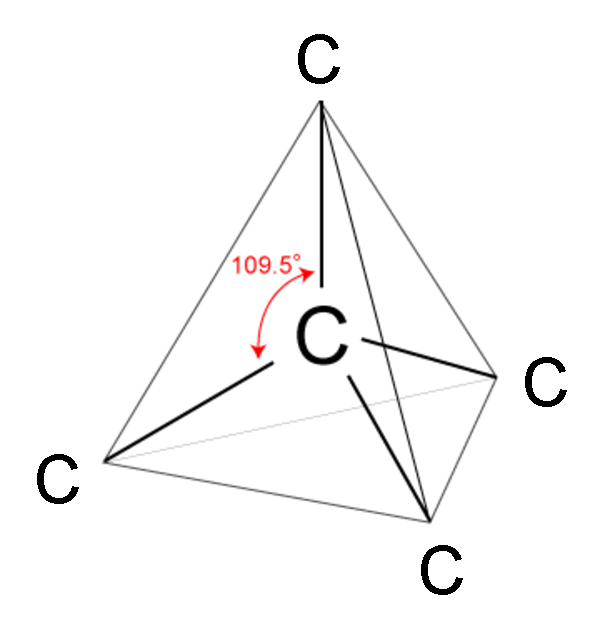
\includegraphics[width= 5 cm]{carbon.eps}
\end{center}

\subsection{幾何学的なやり方}

この正四面体の各頂点を A, B, C, D とし、各辺の長さ(AB, AC, AD, BC, $\cdots$)を 1 とする。
また、重心を G、辺 BC の中点を M とし、さらに、頂点 A から $\bigtriangleup$ BCD に下した垂線の足を K とする。


\begin{center}
	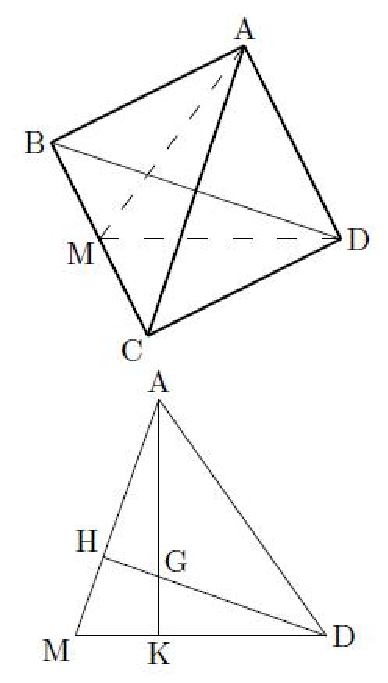
\includegraphics[width= 5 cm]{Carbon_BA.pdf}
\end{center}
この設定の元で、結合角(例えば、$\angle$ AGD)を求めよう。

まず、$\bigtriangleup$ CDM において、$\angle$ DMC = $\perp$, $\angle$ DCM = $60^o$ であるので、
\begin{align*}
{\rm CM} : {\rm CD} : {\rm DM} &= 1: 2 : \sqrt{3} \\
\therefore \quad {\rm DM} &= \dfrac{\sqrt{3}}{2}
\end{align*}

次に、$\bigtriangleup$ KBC に着目すると、$\angle$ BKC = $120^o$ より $\angle$ BKM = $60^o$ であるので MK:KB=1:2 となる。
また、K は $\bigtriangleup$ BCD の重心であるので、KB=KD、したがって、
\begin{align*}
{\rm DM} &= {\rm MK} + {\rm KD} = {\rm MK} + {\rm KB} = 3 \times {\rm MK} \\
\therefore \quad {\rm MK} 
	&=\dfrac{ {\rm DM} }{3} \\
	&=\dfrac{\sqrt{3}}{6}
\end{align*}

AM=DM であることに注意すると、$\bigtriangleup$ AMK において三平方の定理より、
\begin{align*}
{\rm AK} 
	&= \sqrt{ {\rm AM}^2 - {\rm MK}^2 } \\
	&= \dfrac{\sqrt{6}}{3}
\end{align*}

$\bigtriangleup$ AMK $\sim$ $\bigtriangleup$ AGH であるので、AM:AG = AK:AH となり、
\begin{align*}
{\rm AG} 
	&= { {\rm AM} } \times \dfrac{ {\rm AK} }{ {\rm AH} } \\
	&= { {\rm AM} } \times \dfrac{ {\rm AK} }{ ({\rm AM} - {\rm HM}) } \\
	&= \dfrac{\sqrt{3}}{2} \times \dfrac{ \dfrac{\sqrt{6}}{3} }{ \left( \dfrac{\sqrt{3}}{2} - \dfrac{\sqrt{3}}{6} \right) } \\
%	&= \dfrac{\sqrt{3}}{2} \times \dfrac{ \dfrac{\sqrt{6}}{3} }{ \dfrac{2\sqrt{3}}{3} } \\
	&= \dfrac{ \sqrt{6} }{ 4 }
\end{align*}

この時、求める結合角 $\angle$ AGD は、$\bigtriangleup$ AGD に対して余弦定理
\footnote
{
三角形の辺の長さと内角の余弦の間に成り立つ関係を与える定理であり、
$\bigtriangleup$ ABC において、a = BC, b = CA, c = AB, $\alpha$ = $\angle$ CAB, $\beta$ = $\angle$ ABC, $\gamma$ = $\angle$ BCA としたとき
\begin{align*}
a^2 &= b^2 + c^2 − 2 bc \cos \alpha \\
b^2 &= c^2 + a^2 − 2 ca \cos \beta \\
c^2 &= a^2 + b^2 − 2 ab \cos \gamma
\end{align*}
と表される・
}
を適応して、
\begin{align*}
\cos \angle {\rm AGD} 
	&= \dfrac{ {\rm AG}^2 + {\rm GD}^2 - {\rm AD}^2 }{ 2 \times {\rm GA} \times {\rm GD} } \\
	&= \dfrac{ \left( \dfrac{ \sqrt{6} }{ 4 } \right)^2 + \left( \dfrac{ \sqrt{6} }{ 4 } \right)^2 - \left( 1 \right)^2 }{ 2 \times \dfrac{ \sqrt{6} }{ 4 } \times \dfrac{ \sqrt{6} }{ 4 } } \\
%	&= \dfrac{ \dfrac{ 12 }{ 16 } -1 }{\dfrac{ 12 }{ 16 }} \\
	&= -\dfrac{ 1 }{ 3 }
\end{align*}
となる。

関数電卓等を用いて、
\begin{align*}
\angle {\rm AGD} = \cos ^{-1} \left( -\dfrac{1}{3} \right) = 109.4712206 \cdots^o
\end{align*}
という無理数の形で得られるので、これを小数第一位で丸めて、約 $109.5^o$ と表記しているわけである。

\subsection{ベクトル形式での解法}

重心 G から各頂点( A, B, C, D )への長さが 1 の正四面体を考えよう。
これをベクトルで、$\overrightarrow{GA} = {\bm a}, \overrightarrow{GB} = {\bm b}, \cdots$ と表し、
結合角(例えば、$\angle AGB$ )を $\theta$ と表記しよう。

このとき、
\begin{align*}
&{\bm a} \cdot {\bm b} = {\bm a} \cdot {\bm c} = {\bm a} \cdot {\bm d} = {\bm b} \cdot {\bm c} = {\bm b} \cdot {\bm d} = {\bm c} \cdot {\bm d} = 1 \times 1 \times \cos \theta = \cos \theta \\
&|{\bm a}|^2 = |{\bm b}|^2 = |{\bm c}|^2 = |{\bm d}|^2 = 1
\end{align*}
となる。

また、重心の定義より、
\begin{align*}
{\bm a} + {\bm b} + {\bm c} + {\bm d} = {\bm 0} \\
\therefore \quad -{\bm d} ={\bm a} + {\bm b} + {\bm c}
\end{align*}

したがって、
\begin{align*}
|{\bm d} | 
	&= |{\bm a} + {\bm b} + {\bm c}| \\
	&= \sqrt{ |{\bm a}|^2 + |{\bm b}|^2 + |{\bm c}|^2 + 2{\bm a}{\bm b} + 2{\bm a}{\bm c} + 2{\bm b}{\bm c} } \\
	&= \sqrt{ 3 + 6 \cos \theta } \\
	&= 1 \\
\therefore \quad \cos \theta &= -\dfrac{1}{3}
\end{align*}
を得る。

\newpage

\section{自由連結鎖の慣性半径}
\label{sec:rg}

\subsection{慣性半径の定義}

\subsubsection{セグメントの位置ベクトルを用いた定義}
% $\bm{r}_{i}$ 

$0\sim$ N のインデックスを付与した N+1 個のセグメント( N 個のボンド)からなる自由連結鎖を考えよう。
任意の基準点から見た $i$ 番目のセグメントの位置ベクトルを $\bm{r}_i$ で指定した場合、この高分子鎖の重心は、以下のように定義することができる。
\begin{equation*}
\bm{r}_g = \dfrac{1}{N+1} \sum_{j=0}^{N} \bm{r}_j
\end{equation*}

このとき、慣性半径 $R_g$ は、鎖の重心 $\bm{r}_g$ から各セグメントまでの距離の二乗平均の平方根として以下のように定義される。
\begin{equation*}
R_g^2 = \dfrac{1}{N+1} \left\langle \sum_{i=0}^{N} |\bm{r}_i - \bm{r}_g|^2 \right\rangle
\end{equation*}

この定義は、セグメントの重量を単位量 1 と見た場合の、剛体の力学における慣性モーメントと同等であると考えれば理解しやすい。

\subsubsection{二体間距離を用いた定義}
% $\bm{r}_{i} - \bm{r}_{j}& 

上記の重心からの定義式を、ボンドベクトルを用いて表現できるセグメント間の二体間距離によって書き換えることを考えよう。
位置ベクトル $\bm{r}_{i}, \bm{r}_{j}$ で表される任意の二つのセグメント $i, j$ 間の距離の二乗 $|\bm{r}_{i} - \bm{r}_{j}|^2$ は、もう一つの点を想定した三角形の余弦定理により、以下のように書ける。 
\begin{align*}
|\bm{r}_{i} - \bm{r}_{j}|^2 = |\bm{r}_{i}|^2 - 2 \bm{r}_{i}\cdot\bm{r}_{j} + |\bm{r}_{j}|^2
\end{align*}
ここで、上記の三角形の一点を重心であると考えれば、余弦定理を用いて、慣性半径の二乗平均 $R_g^2$を二体間距離、すなわち、ボンドベクトルの結合で定義できることになる。

それぞれのセグメントの位置ベクトルの基準を重心 $\bm{r}_g$ とした上で、各セグメントの距離をすべて積算するために、上式の左辺の二重和をとると、以下のように展開できる。
\begin{align*}
\sum_{i = 0}^N \sum_{j=0}^N \left| \bm{r}_i - \bm{r}_j \right|^2
	&= \sum_{i = 0}^N \sum_{j=0}^N  \left| (\bm{r}_i - \bm{r}_g) - (\bm{r}_j - \bm{r}_g) \right|^2 \\
	&= \sum_{i = 0}^N \sum_{j=0}^N \left[ \left| \bm{r}_i - \bm{r}_g \right|^2 + \left|\bm{r}_j - \bm{r}_g \right|^2 
		-2 (\bm{r}_i - \bm{r}_g) \cdot (\bm{r}_j - \bm{r}_g) \right] \\
	&= \sum_{i = 0}^N \sum_{j=0}^N \left| \bm{r}_i - \bm{r}_g \right|^2 + \sum_{i = 0}^N \sum_{j=0}^N \left|\bm{r}_j - \bm{r}_g \right|^2 
		-2 \sum_{i = 0}^N \sum_{j=0}^N (\bm{r}_i - \bm{r}_g) \cdot (\bm{r}_j - \bm{r}_g)
\end{align*}

ここで、第一項及び第二項の二重和は、因子中に存在しないダミー変数(第一項では $j$)の分だけ総和を取る( $N+1$ 個足し合わせる)ことができるので、
\begin{align*}
\sum_{i = 0}^N \sum_{j=0}^N \left| \bm{r}_i - \bm{r}_g \right|^2 
	&= \sum_{i = 0}^N \left[ \underbrace{ \left| \bm{r}_i - \bm{r}_g \right|^2 + \left| \bm{r}_i - \bm{r}_g \right|^2 + \cdots + \left|\bm{r}_i - \bm{r}_g \right|^2 }_{N+1} \right]\\
	&= (N+1) \sum_{i = 0}^N \left| \bm{r}_i - \bm{r}_g \right|^2 \\
\end{align*}

また、第三項のそれぞれの因子は以下のように展開すれば 0 となる。
\begin{align*}
\sum_{i=0}^N (\bm{r}_i - \bm{r}_g) 
	&= \left[ \underbrace{ (\bm{r}_0 - \bm{r}_g) + (\bm{r}_1 - \bm{r}_g) + \cdots + (\bm{r}_N - \bm{r}_g) }_{N+1}\right] \\
	&= \sum_{i=0}^N \bm{r}_i -(N+1) \bm{r}_g \\
	&= \sum_{i=0}^N \bm{r}_i -(N+1) \dfrac{1}{N+1} \sum_{i=0}^{N} \bm{r}_i \\
	&=0
\end{align*}

上記の結果を代入して、カッコ内の第二項のダミー変数 $j$ を $i$ と書き換えることで、以下の表式を得る。
\begin{align*}
\sum_{i = 0}^N \sum_{j=0}^N \left| \bm{r}_i - \bm{r}_j \right|^2
	&= (N + 1) \left[ \sum_{i=0}^N \left| \bm{r}_i - \bm{r}_g \right|^2 + \sum_{j=0}^N \left| \bm{r}_j - \bm{r}_g \right|^2 \right] -2 \sum_{i=0}^N (\bm{r}_i - \bm{r}_g) \sum_{j=0}^N (\bm{r}_j - \bm{r}_g) \\
	&= 2(N + 1) \sum_{i=0}^N (\bm{r}_i- \bm{r}_g)^2 \\
\therefore \sum_{i=0}^N (\bm{r}_i- \bm{r}_g)^2 
	&= \dfrac{1}{2(N+1)} \sum_{i = 0}^N \sum_{j=0}^N \left| \bm{r}_i - \bm{r}_j \right|^2
\end{align*}

したがって、上記を用いて、慣性半径は二体間距離を用いた形で、以下のように表記できることが確認できた。
\begin{align*}
R_g^2 
	&= \dfrac{1}{N+1} \left\langle \sum_{i=0}^{N} |\bm{r}_i - \bm{r}_g|^2 \right\rangle \\
	&= \dfrac{1}{2(N+1)^2} \left \langle \sum_{i=0}^N \sum_{j=0}^N \left| \bm{r}_i - \bm{r}_j \right|^2 \right \rangle
\end{align*}

なお、ここで行ってきた議論は、高分子鎖の性質に依らないものであり、汎用性を持った表記となっている。

\subsection{自由連結鎖の慣性半径}

次に、自由連結鎖を想定して、下式を具体的に展開しよう。
\begin{equation*}
R_g^2 = \dfrac{1}{2(N+1)^2} \left \langle \sum_{i=0}^N \sum_{j=0}^N \left| \bm{r}_i - \bm{r}_j \right|^2 \right \rangle
\end{equation*}

\subsubsection{場合分け}

二重和を展開するために、セグメントの位置関係を場合分けすると、以下に示したように二つの場合に分けて考えることができる。

\begin{itemize}
\item
$i < j$ の場合

%\setlength\unitlength{1truecm}
%\begin{picture}(12,2)(0,0)
%\linethickness{0.5pt}
%\put(1,1){\line(1,0){10}}
%\linethickness{3pt}
%\put(4,1){\line(1,0){4}}
%\put(1, 1){\circle*{0.4}}
%\put(4, 1){\circle*{0.4}}
%%\put(6, 1){\circle*{0.4}}
%\put(8, 1){\circle*{0.4}}
%\put(11, 1){\circle*{0.4}}
%%
%\put(0.9,0.5){$0$}
%\put(3.9,0.5){$i$}
%%\put(5.9,0.5){$i$}
%\put(7.9,0.5){$j$}
%\put(10.8,0.5){$N$}
%\end{picture}

ここで、考察の対象としているのは自由連結鎖(暗黙の内に理想鎖として取り扱い、長距離相互作用(排除体積効果)も無視している)であるから、$0 \sim i$ および $j \sim N$ のセグメントをつなげた部分鎖については、隣同士のセグメントを結合するボンドのボンドベクトルのアンサンブル平均は $\bm{0}$ となる。
したがって、$i$ 番目のセグメントから、$j$ 番目のセグメントまでの部分鎖中のボンドベクトルだけを考えればよいことになる。

\item
$j < i$ の場合

%\setlength\unitlength{1truecm}
%\begin{picture}(12,2)(0,0)
%\linethickness{0.5pt}
%\put(1,1){\line(1,0){10}}
%\linethickness{3pt}
%\put(4,1){\line(1,0){4}}
%\put(1, 1){\circle*{0.4}}
%\put(4, 1){\circle*{0.4}}
%%\put(6, 1){\circle*{0.4}}
%\put(8, 1){\circle*{0.4}}
%\put(11, 1){\circle*{0.4}}
%%
%\put(0.9,0.5){$0$}
%\put(3.9,0.5){$j$}
%%\put(5.9,0.5){$i$}
%\put(7.9,0.5){$i$}
%\put(10.8,0.5){$N$}
%\end{picture}

$i,j$ の大小関係が反転したこちらの場合においても、条件は上記の場合とまったく同一となる。
\end{itemize}

結局、上記二種類の等価な相関を考えればよいので、例えば、 $i < j$ の場合だけを考えて 2 倍すればよいことになる。

\subsubsection{ボンドベクトルへの変換}

理想鎖において、注目する部分鎖中の任意の二つのボンドベクトルを新たなダミー変数を用いて $\bm{u}_k$ および $\bm{u}_l$ と表した場合、各ボンドの方向は無相関であるから、
\begin{align*}
\langle \bm{u}_k \cdot \bm{u}_l \rangle 
	&= \langle \bm{\hat{u}}_k \cdot \bm{\hat{u}}_l \rangle a^2 \\
	&=
\begin{cases}
\langle |\bm{\hat{u}}_k |^2 \rangle a^2 = a^2	&\quad (\text{$k = l$ のとき}) \\
\langle \bm{u}_k \rangle \cdot \langle \bm{u}_l \rangle = \bm{0}\cdot\bm{0} = 0	&\quad(\text{$k \neq l$ のとき})
\end{cases}
\end{align*}
となる。
ここで、$\bm{\hat{u}}_k \equiv \dfrac{\bm{u}_k}{|\bm{u}_k|}$ は $\bm{u}_k$ 方向の単位ベクトル、$a$ はボンドの長さを表している。

この関係を用いて、セグメント間の二体間距離をボンドベクトルへと変換すると、以下のように展開することができる。
\begin{align*}
\left \langle \left | \bm{r}_i - \bm{r}_j \right |^2 \right \rangle
	&= \left \langle \left | (\bm{r}_{i+1} - \bm{r}_i) + (\bm{r}_{i+2} - \bm{r}_{i+1}) + \cdots + (\bm{r}_j - \bm{r}_{j-1}) \right |^2 \right \rangle \\
	&= \left \langle \left | \bm{u}_i + \bm{u}_{i+1} + \cdots + \bm{u}_{j-1} \right |^2 \right \rangle \\
	&= \left \langle \left| \sum_{k=i}^{j-1} \bm{u}_{k} \right|^2 \right\rangle \\
	&= \sum_{k=i}^{j-1} \left \langle \left| \bm{u}_{k} \right|^2 \right\rangle + \sum_{k \neq l} \left \langle \bm{u}_{k} \cdot \bm{u}_{l} \right\rangle \\
	&= a^2(j-i)
\end{align*}


\subsubsection{具体的な展開}


上式の関係を利用して、結局、二つのセグメント間の距離からの慣性半径の表式を展開して、
\begin{align*}
R_g^2 
	&= \dfrac{1}{2(N+1)^2} \left \langle \sum_{i=0}^N \sum_{j=0}^N \left|\bm{r}_i - \bm{r}_j \right|^2 \right \rangle\\
	&= \dfrac{1}{2(N+1)^2} \left \langle 2 \sum_{i=0}^N \sum_{j=0}^{i-1} \left|\bm{r}_i - \bm{r}_j \right|^2 \right \rangle\\
	&= \dfrac{a^2}{(N+1)^2} \sum_{i=0}^N \sum_{j=0}^{i-1} (i -j) \\
	&= \dfrac{a^2}{(N+1)^2} \sum_{i=0}^N \left[ \underbrace{(i -0) +(i -1) + \cdots + (i -\{i-1\} ) }_i \right]\\
	&= \dfrac{a^2}{(N+1)^2} \sum_{i=0}^N \left[ \underbrace{(i+i+ \cdots +i ) }_i - \underbrace{(0+1+ \cdots + \{i-1\} ) }_i\right]\\
	&= \dfrac{a^2}{(N+1)^2} \sum_{i=0}^N \left[ i^2 - \sum_{k=0}^{i-1} k \right]
\end{align*}
二行目へは $j < i$ の場合だけを対象として総和を分割したうえで因子を二倍しており、三行目へはボンドベクトルに変換することで上述の関係を用いている。
さらに、四行目への展開で $j$ に関する総和を取ってから、まとめなおしている。

累乗の和に関する公式
\footnote{
累乗の和に関する公式は、以下のようになっている。
\begin{equation*}
\begin{cases}
\displaystyle \sum_{i=0}^{N} i = \dfrac{1}{2} N (N+1) \\[12pt]
\displaystyle \sum_{i=0}^{N} i^2 = \dfrac{1}{6} N (N+1)(2N+1)
%\\[12pt]
%\displaystyle \sum_{i=0}^{N} i^3 = \left\{\dfrac{1}{2} N (N+1) \right\}^2
\end{cases}
\end{equation*}
}
を用いることで、上式はさらに展開できる。
\begin{align*}
R_g^2
	&= \dfrac{a^2}{(N+1)^2} \sum_{i=0}^N \left[ i^2 - \sum_{k=0}^{i-1} k \right] \\
	&= \dfrac{a^2}{(N+1)^2} \sum_{i=0}^N \left[ i^2 - \left\{ \dfrac{1}{2} \left(i-1 \right) i \right\} \right] \\
	&= \dfrac{a^2}{2(N+1)^2} \sum_{i=0}^N (i^2 + i) \\
	&= \dfrac{a^2}{2(N+1)^2} \left[ \left\{ \dfrac{1}{6} N (N+1)(2N+1) \right\} + \left\{ \dfrac{1}{2} N (N + 1) \right\} \right] \\
	&= \dfrac{a^2 N(N+1)}{12(N+1)^2} [( 2N +1) +3] \\
	&= \dfrac{N(N+1)(N+2) }{6(N+1)^2} a^2\\
	&\simeq \dfrac{N}{6} a^2
\end{align*}
なお、二行目では初項 $0$、末項 $i-1$ として公式を用いており、最終行へは $N \gg 1$ であることから、$\dfrac{(N+1)(N+2) }{(N+1)^2}\simeq 1$ とした。

%\vspace{10pt}

\subsection{積分形式での展開}


上式は、離散的な和の形で表して公式を利用して解いているが、一般的に積分の形で書くと以下のようになる。

なお、こちらの展開においては、上記の展開で行った $i , j$ の大小関係に基づく絶対値の場合分けを積分範囲の分割という形で行っているので、式中には 2 の因子はでてこない。
\begin{align*}
R_g^2 
	&= \dfrac{1}{2(N+1)^2} \left \langle \int_{0}^N \odif{i} \int_{0}^N \odif{j} (\bm{r}_i - \bm{r}_j) \cdot (\bm{r}_i - \bm{r}_j) \right \rangle\\
	&= \dfrac{1}{2(N+1)^2} \left \langle \int_{0}^N \odif{i} \int_{0}^{N} \odif{j} \left|\bm{r}_i - \bm{r}_j \right|^2 \right \rangle\\
	&= \dfrac{a^2}{2(N+1)^2} \int_{0}^N \odif{i} \int_{0}^{N} \odif{j} \left|\bm{r}_i - \bm{r}_j \right| \\
	&= \dfrac{a^2}{2(N+1)^2} \int_{0}^N \odif{i} \left\{ \int_{0}^{i} \odif{j} (i -j) + \int_i^N \odif{j} \left[ -(i-j) \right] \right\} \\
	&= \dfrac{a^2}{2(N+1)^2} \int_{0}^N \odif{i} \left\{ \left [ij - \dfrac{j^2}{2} \right]_0^i - \left[ ij - \dfrac{j^2}{2} \right]_i^N \right\} \\
	&= \dfrac{a^2}{2(N+1)^2} \int_{0}^N \odif{i} \left\{ \left (i^2 - \dfrac{i^2}{2} \right) - \left[ \left(Ni - \dfrac{N^2}{2} \right) - \left (i^2 - \dfrac{i^2}{2} \right) \right] \right\} \\
	&= \dfrac{a^2}{2(N+1)^2} \int_{0}^N \odif{i} \left\{ i^2 - Ni + \dfrac{N^2}{2} \right\} \\
	&= \dfrac{a^2}{2(N+1)^2} \left[ \dfrac{i^3}{3} - \dfrac{N}{2}i^2 + \dfrac{N^2}{2} i \right]_0^N \\
	&= \dfrac{a^2}{2(N+1)^2} \left( \dfrac{N^3}{3} - \dfrac{N^3}{2} + \dfrac{N^3}{2} \right) \\
	&= \dfrac{N^3 }{6(N+1)^2} a^2\\
	&\simeq \dfrac{N}{6} a^2\\
\end{align*}
\newpage

\section{自由回転鎖モデルの二乗平均末端間距離}
\label{sec:1FR_R2}

\subsection{自由回転鎖モデルの一般化したボンドベクトルの内積}

自由回転鎖において、隣接するボンドベクトルの内積のアンサンブル平均は、それらのベクトルの成す角 $\theta$ を用いて、
\begin{align*}
	\langle \bm{u}_i \cdot \bm{u}_{i+1} \rangle = a^2 \cos \theta 
\end{align*} 
と書くことができる。
この表式は、内積を取る一方のベクトルを他方に射影した長さ $a \cos \theta$ と、もう一方のベクトルの長さ $a$ とのスカラー積であると考えることができる。

したがって、一つ離れたボンドベクトル $\bm{u}_{i+2}$ との内積は、離れたベクトル $\bm{u}_{i+2}$ を隣接するベクトル $\bm{u}_{i+1}$ に射影し、さらに、その射影を考えればよいので、
\begin{align*}
	\langle \bm{u}_i \cdot \bm{u}_{i+2} \rangle 
		&= a^2 \cos^2 \theta 
\end{align*}
となる。

ここで、$p=\cos \theta$ として、さらに一般化すると、$k$(ただし、$k$ は正の整数)だけ離れたボンドベクトルの内積は
\begin{align}
	\langle \bm{u}_i \cdot \bm{u}_{i+k} \rangle 
		&= a^2 \cos^k \theta \notag \\
		&= a^2 p^k 
\label{eq:naiseki}
\end{align}
と記述することができる。

\subsection{自由回転鎖モデルの二乗平均末端間距離}

自由連結鎖の二乗平均末端間距離 $\langle \bm{R}^2 \rangle$ は、
平均二乗末端間距離 $R^2$ は、末端間ベクトルの大きさの二乗のアンサンブル平均として、以下のように展開できる。
\begin{align*}
	R^2
		&= \langle |\bm{R}|^2 \rangle \notag \\
		&= \langle |\bm{u}_0 + \bm{u}_1 + \cdots + \bm{u}_{N-1}|^2 \rangle \notag \\
		&= 
			[ 
			{\color{red} |\bm{u}_0|^2} + \langle \bm{u}_0 \cdot \bm{u}_1 \rangle + \langle \bm{u}_0 \cdot \bm{u}_2 \rangle + \cdots + \langle \bm{u}_0 \cdot \bm{u}_{N-1} \rangle 
			] \notag \\
		&\quad+ 
			[ 
			\langle \bm{u}_1 \cdot \bm{u}_0 \rangle + {\color{red} |\bm{u}_1|^2} + \langle \bm{u}_1 \cdot \bm{u}_2 \rangle + \cdots + \langle \bm{u}_1 \cdot \bm{u}_{N-1} \rangle 
			] \notag \\
		&\quad\quad \vdots \notag \\
		&\quad+ 
			[ 
			\langle \bm{u}_{N-1} \cdot \bm{u}_0 \rangle + \langle \bm{u}_{N-1} \cdot \bm{u}_1 \rangle + \cdots + \langle \bm{u}_{N-1} \cdot \bm{u}_{N-2} \rangle + {\color{red} |\bm{u}_{N-1}|^2} 
			] \notag \\
%%
		&= 
			[ 
			|\bm{u}_0|^2 +  |\bm{u}_1|^2 + \cdots + |\bm{u}_{N-1}|^2 
			] \notag \\
		&\quad+		
			[
			{\color{blue} \langle \bm{u}_0 \cdot \bm{u}_1 \rangle} + {\color{green} \langle \bm{u}_0 \cdot \bm{u}_2 \rangle} + \cdots + \langle \bm{u}_0 \cdot \bm{u}_{N-1} \rangle 
			] \notag \\
		&\quad+ 
			[ 
			{\color{blue} \langle \bm{u}_1 \cdot \bm{u}_0 \rangle} +\langle \bm{u}_1 \cdot \bm{u}_2 \rangle + \cdots + \langle \bm{u}_1 \cdot \bm{u}_{N-1} \rangle 
			] \notag \\
		&\quad+ 
			[ 
			{\color{green} \langle \bm{u}_2 \cdot \bm{u}_0 \rangle} +\langle \bm{u}_2 \cdot \bm{u}_1 \rangle + \cdots + \langle \bm{u}_2 \cdot \bm{u}_{N-1} \rangle 
			] \notag \\
		&\quad\quad \vdots \notag \\
		&\quad+ 
			[ 
			\langle \bm{u}_{N-1} \cdot \bm{u}_0 \rangle + \langle \bm{u}_{N-1} \cdot \bm{u}_1 \rangle + \cdots + \langle \bm{u}_{N-1} \cdot \bm{u}_{N-2} \rangle
			] \notag \\
%%
		&= 
			[ 
			|\bm{u}_0|^2 +  |\bm{u}_1|^2 + \cdots + |\bm{u}_{N-1}|^2 
			] \notag \\
%
		&\quad+		
			2[
			\langle \bm{u}_0 \cdot \bm{u}_1 \rangle + \langle \bm{u}_0 \cdot \bm{u}_2 \rangle + \cdots + \langle \bm{u}_0 \cdot \bm{u}_{N-1} \rangle 
			] \notag \\
		&\quad+ 
			2[ 
			\langle \bm{u}_1 \cdot \bm{u}_2 \rangle +\langle \bm{u}_1 \cdot \bm{u}_3 \rangle + \cdots + \langle \bm{u}_1 \cdot \bm{u}_{N-1} \rangle 
			] \notag \\
		&\quad+ 
			2[ 
			\langle \bm{u}_2 \cdot \bm{u}_3 \rangle +\langle \bm{u}_2 \cdot \bm{u}_4 \rangle + \cdots + \langle \bm{u}_2 \cdot \bm{u}_{N-1} \rangle 
			] \notag \\
		&\quad\quad \vdots \notag \\
		&\quad+ 
			2\langle \bm{u}_{N-2} \cdot \bm{u}_{N-1} \rangle
			\notag \\
%
%
		&= \sum_{i=0}^{N-1} \left \langle \left| \bm{u}_{i} \right|^2 \right\rangle + 2 \sum_{i=0}^{N-2} \sum_{j=i+1}^{N-1} \langle \bm{u}_i \cdot \bm{u}_j \rangle
\end{align*}
であった。

上式の第二項に、(\ref{eq:naiseki}) 式を代入すると、
\begin{align*}
\sum_{i=0}^{N-2} \sum_{j=i+1}^{N-1} \langle \bm{u}_i \cdot \bm{u}_j \rangle 
	&= \sum_{i=0}^{N-2} a^2 (p + p^2 + \cdots + p^{i+1} ) \notag \\
	&= a^2 \sum_{i=0}^{N-2}  \dfrac{p(1-p^{i+1})}{1-p} \notag \\
	&= a^2 \dfrac{p}{1-p} \sum_{i=0}^{N-2}  (1-p^{i+1}) \notag \\
	&= a^2 \dfrac{p}{1-p} \left \{ \sum_{i=0}^{N-2} 1 - \sum_{i=0}^{N-2} (p^{i+1}) \right \} \notag \\
	&= a^2 \dfrac{p}{1-p} \left\{ (N-1) - \dfrac{p(1-p^{N-1})}{1-p} \right \} \notag \\
	&= Na^2 \dfrac{p}{1-p} - a^2 \dfrac{p}{1-p} - a^2 \dfrac{p^2(1-p^{N-1})}{(1-p)^2} \notag \\
	&= Na^2 \dfrac{p}{1-p} - a^2 \dfrac{p(1-p)}{(1-p)^2} - a^2 \dfrac{p^2(1-p^{N-1})}{(1-p)^2} \notag \\
	&= Na^2 \dfrac{p}{1-p} - a^2 \dfrac{p(1-p^{N})}{(1-p)^2}
\end{align*}
と展開することができる。

したがって、自由回転鎖モデルの二乗平均末端間距離 $\langle \bm{R}_{fr}^2 \rangle$ は、
\begin{align*}
	\langle \bm{R}_{fr}^2 \rangle
		&= N a^2 + 2Na^2 \dfrac{p}{1-p} -2a^2 \dfrac{p(1-p^{N})}{(1-p)^2} \notag \\
		&= N a^2 \left \{ \dfrac{1+p}{1-p} - \dfrac{2}{N} \dfrac{p(1-p^{N})}{(1-p)^2} \right \}
% \notag \\
%		&\simeq N a^2 \dfrac{1+p}{1-p} \quad\quad \Big( \because \text{N が大きくなれば、第二項} \rightarrow 0 \Big) \notag \\
%		&= N a^2 \dfrac{1+\cos \theta}{1-\cos \theta}
\end{align*}

ここで、$N \rightarrow \infty$ の場合に、第二項は無視できるようになるので、結局、
\begin{align*}
	\langle \bm{R}_{fr}^2 \rangle
		&\simeq N a^2 \dfrac{1+p}{1-p} \notag \\
		&= N a^2 \dfrac{1+\cos \theta}{1-\cos \theta}
\end{align*}

\newpage

\section{一次元自由連結鎖モデルについて}
\label{sec:1DRW}

\subsection{一次元自由連結鎖の末端間距離 $R$ の分布関数 $P(R)$}
\label{ssec:1DRW_PR}

$N+1$ 個のセグメントが長さ $b$ である $N$ 個のボンドで連結された自由連結鎖が一次元に伸びた一次元ポリマーを考えてみよう。
なお、各セグメント間をつなぐボンドの向きを考え、それぞれの方向(伸長方向の任意の向きを状態 A とし、その逆向きを状態 B とする)へのボンドの出現確率が共に等しい(1/2)だとする。
これは、一次元のランダムウォークモデルと等価である。
このとき、末端間距離 $R$ の分布関数 $P(R)$ は、二項分布
\footnote
{
二項分布の定義及びその性質については、
\href{https://dl.dropboxusercontent.com/u/18899343/Probability/Prob_Dist/Prob_Dist.pdf}{「分布関数」}
を参照していただきたい。
}に従うと考えることができる。

ポリマー鎖の末端間距離が $R = Xb$ となるのは、状態 A となるボンドの数 $n_A$ が、状態 B となるボンドの数 $n_B$ よりも $X$ 個分だけ偏っている(多い、あるいは少ない)という状態であり、それぞれの状態のボンドの数は、以下となる
\footnote
{
なお、 $n_A$ と $n_B$ の分子における $X$ の因子の符号が逆転していることに注意されたい。
これは、絶対値を外すときに生じたものである。
}。
\begin{align*}
\begin{cases}
n_A +n_B = N \\[8pt]
| n_A - n_B | = X
\end{cases}\\[10pt]
\therefore
\begin{cases}
n_A = \dfrac{N \pm X}{2} \\[8pt]
n_B = \dfrac{N \mp X}{2}
\end{cases}
\end{align*}

したがって、末端間距離 $R$ の分布関数 $P(R)$ は、「ボンドの総数 $N$ から状態 A であるボンドを上式を満たすようなボンドの数 $n_A$ だけ選び取り、残りを状態 B に選び出す」という事象の確率で表されることになり、以下のように、確率変数として $n_A$ を用いた形で書くことができる。
\begin{align*}
P(R)
	&= {}_N C_{n_A} \left(\dfrac{1}{2} \right)^{n_A} \left(\dfrac{1}{2} \right)^{N-n_A} \notag \\
	&= {}_N C_{n_A} \left(\dfrac{1}{2} \right)^N \\
	&= P(n_A)
\end{align*}

\subsection{一次元自由連結鎖の二乗平均末端間距離 $\langle R^2 \rangle$}
\label{ssec:1DRW_R2}

上記の確率分布関数を用いて、二乗平均末端間距離 $\langle R^2 \rangle$ は以下のように展開できる。
\begin{align*}
\langle R^2 \rangle 
	&= \sum_{n_A = 0}^{N} R^2 P(R) \notag \\
	&= \sum_{n_A = 0}^{N} (Xb)^2 \times P(n_A) \notag \\
	&= b^2 \sum_{n_A = 0}^{N} (2n_A - N)^2 \times P(n_A) \notag \\
	&= b^2 \sum_{n_A = 0}^{N} (4n_A^2 -4Nn_A + N) \times P(n_A) \notag \\
	&= b^2 \left[ 4 \sum_{n_A = 0}^{N} n_A^2 \times P(n_A) - 4N\sum_{n_A = 0}^{N} n_A \times P(n_A) + N^2 \sum_{n_A = 0}^{N} P(n_A) \right]
\end{align*}

ここで、括弧内の各項の因子を確認しよう。

第二項 $\displaystyle \sum_{n_A = 0}^{N} n_A \times P(n_A)$ は期待値 $E(n_A)$、第三項は確率分布の全範囲にわたる総和であるから、$\displaystyle \sum_{n_A = 0}^{N} P(n_A) =1$ である。
なお、第一項の $\displaystyle \sum_{n_A = 0}^{N} n_A^2 \times P(n_A)$ は、分散 $V(n_A)$ を用いて、以下のように書くことができる
\footnote
{
分散の定義から、以下の関係を導出できる。
\begin{align*}
V(n_A)
	&=E(n_A^2) \\
	&=\sum [n_A - E(n_A)]^2 P(n_A)\\
	&=\sum [n_A^2 -2 n_A E(n_A) + E(n_A)^2] P(n_A)\\
	&=\sum n_A^2 P(n_A) -2 E(n_A) \sum n_A P(n_A) + E(n_A)^2 \sum P(n_A) \\
	&=\sum n_A^2 P(n_A) -2 E(n_A) E(n_A) + E(n_A)^2 \\
	&=\sum n_A^2 P(n_A) - E(n_A)^2 \\
\therefore \quad &\sum n_A^2 P(n_A) = V(n_A) + E(n_A)^2
\end{align*}
}。
\begin{align*}
\displaystyle \sum_{n_A = 0}^{N} n_A^2 \times P(n_A)
	= V(n_A)+E(n_A)^2
\end{align*}


それぞれの事象の確率が 1/2 であった場合の二項分布における期待値 $E(n_A)$、および分散 $V(n_A)$ は、それぞれ、以下であった
\footnote
{
この導出については、
\href{https://dl.dropboxusercontent.com/u/18899343/Probability/Prob_Dist/Prob_Dist.pdf}{「分布関数」}
を参照されたい。
}。
\begin{align*}
\begin{cases}
E(n_A)=\dfrac{N}{2} \\[8pt]
V(n_A)=\dfrac{N}{4}
\end{cases}
\end{align*}

したがって、求める二乗平均末端間距離 $\langle R^2 \rangle$ は、
\begin{align*}
\langle R^2 \rangle 
	&= b^2 \left[ 4 \{V(n_A)+E(n_A)^2\} - 4N E(n_A) + N^2 \right] \\
	&= b^2 [ (N +N^2) - 2N^2 + N^2 ] \\
	&= N b^2
\end{align*}
となる。

\subsection{一次元自由連結鎖のエントロピー}
\label{ssec:1DRW_S}

自由連結鎖の末端間距離が $R$ となるようなボンドの微視的状態数 $W(R)$ は、前述の確率 $P(R)$ から規格化因子である $(1/2)^N$ を除いて、以下のように書くことができる。
\begin{align*}
W 
	&= {}_N C_{n_A} \\
	&= \dfrac{N!}{(N-n_A)! n_A!} \\[8pt]
	&= \dfrac{N!}{n_A! n_B!} \\
	&= \dfrac{N!}{ \left( \dfrac{N + X}{2} \right)! \left( \dfrac{N - X}{2} \right)!}
\end{align*}

ボルツマンの関係式によれば、微視的状態数 $W$ を用いて、エントロピー $S$ は、
\begin{align*}
S=k_B \ln W
\end{align*}
で表されるので、上記のボンドの微視的状態数 $W$ を用いて、
\begin{align*}
S 
	&= k_B \ln W \\
	&= k_B \ln \left[ \dfrac{N!}{ \left( \dfrac{N+X}{2} \right)! \left( \dfrac{N-X}{2} \right)!} \right] \\
	&= k_B \left[ \ln N! -\ln \left( \dfrac{N+X}{2}\right)! -\ln \left( \dfrac{N-X}{2}\right)! \right]
\end{align*}
となる。

ここで、スターリングの公式
\begin{align*}
\ln n! \simeq n \ln n -n
\end{align*}
を用いて、上式は、以下のように展開できる。

\begin{align*}
S 
	&\simeq k_B \left[ \{ N\ln N - N \} - \left\{ \left( \dfrac{N+X}{2} \right)\ln \left( \dfrac{N+X}{2} \right) -\left( \dfrac{N+X}{2} \right) \right\} \right. \\
		&\quad \quad \left. - \left\{ \left( \dfrac{N-X}{2}\right) \ln \left( \dfrac{N-X}{2} \right) - \left( \dfrac{N-X}{2} \right) \right\} \right]\\
	&= k_B \left[ N\ln N - \left( \dfrac{N+X}{2} \right)\ln \left( \dfrac{N+X}{2}\right) - \left( \dfrac{N-X}{2} \right) \ln \left( \dfrac{N-X}{2} \right) \right]\\
	&= k_B \left[ N\ln N - \dfrac{N}{2} \ln \left( \dfrac{N+X}{2} \right)\left( \dfrac{N-X}{2} \right) 
		- \dfrac{X}{2} \ln \dfrac{\left( \dfrac{N+X}{2}\right)}{ \left( \dfrac{N-X}{2} \right) } \right]  \\
	&= k_B \left[ N\ln N - \dfrac{N}{2} \ln \left( \dfrac{N^2-X^2}{4} \right) - \dfrac{X}{2} \ln \dfrac{N + X}{ N - X } \right]  \\
	&= k_B \left[ N\ln N - \dfrac{N}{2} \ln \left\{ \dfrac{N^2}{4}\left(1-\dfrac{X^2}{N^2} \right) \right\} 
	- \dfrac{X}{2} \ln \left( 1 + \dfrac{2X}{N-X} \right) \right]  \\
	&= k_B \left[ N\ln N - \dfrac{N}{2} \ln \dfrac{N^2}{4} - \dfrac{N}{2} \ln \left(1-\dfrac{X^2}{N^2} \right) 
	- \dfrac{X}{2} \ln \left( 1 + \dfrac{2X}{N-X} \right) \right]  \\
	&\simeq k_B \left[ N\ln N - \dfrac{N}{2} \ln \dfrac{N^2}{4} - \dfrac{N}{2}\left(-\dfrac{X^2}{N^2} \right) 
	- \dfrac{X}{2} \left(\dfrac{2X}{N-X} \right) \right]  \\
	&= k_B \left( N\ln N - \dfrac{N}{2} \ln \dfrac{N^2}{4} + \dfrac{X^2}{2N} -\dfrac{X^2}{N - X} \right) \\
	&\simeq k_B \left( N\ln N - \dfrac{N}{2} \ln \dfrac{N^2}{4} + \dfrac{X^2}{2N} -\dfrac{X^2}{N} \right) \\
	&= k_B \left( N\ln N - \dfrac{N}{2} \ln \dfrac{N^2}{4} - \dfrac{X^2}{2N} \right)
\end{align*}
なお、7 行目への展開において、$N \gg X$ と仮定して、対数のテイラー展開を一次の項で打ち切る近似($\ln(1+x) \simeq x$)を行い、さらに9行目で、$\dfrac{X^2}{N-X} = \dfrac{X^2}{N}$ という近似も行った。

したがって、自由連結鎖の一次元モデルのエントロピーは、末端間距離 $R$ が $Xb$ と等しいことから $X = \dfrac{R}{b}$ となることを用いて、$R$ の関数として以下のように表記することができる。
\begin{align*}
S(R)
	&= k_B \left( N\ln N - \dfrac{N}{2} \ln \dfrac{N^2}{4} - \dfrac{R^2}{2Nb^2} \right) \\
	&= C -\dfrac{ k_B}{2Nb^2}R^2 \quad \text{(ただし、$C$ は鎖長 $N$ に依存する定数項)}
\end{align*}

%\subsection{一次元自由連結鎖モデルによるゴム弾性}
%\label{ssec:1DRW_RE}
%
%ここで対象としている自由連結鎖モデルにおいては、内部エネルギー $E$ の寄与のない理想状態を考えているので、末端間距離が $R$ である場合の Helmholtz の自由エネルギー $F(R)$ は、上述のエントロピー $S(R)$ を用いて、以下のように導出される。
%\begin{align*}
%F 	&= E - TS(R) \\
%	&= -TS(R) \\
%	&= -k_B T \left( N\ln N - \dfrac{N}{2} \ln \dfrac{N^2}{4} - \dfrac{R^2}{2Nb^2} \right) 
%\end{align*}
%
%したがって、高分子鎖の末端間距離 $R$ を変化させた場合に、鎖に生じる張力 $f(R)$は、上記の自由エネルギー $F(R)$ を末端間距離 $R$ で微分した形で、
%\begin{align*}
%f(R) 	
%&= \left(\dfrac{\partial F(R)}{\partial R} \right)_T \\
%	&=\dfrac{\partial}{\partial R} \left[ -k_B T \left( N\ln N - \dfrac{N}{2} \ln \dfrac{N^2}{4} - \dfrac{R^2}{2Nb^2} \right) \right]\\
%	&=- \dfrac{k_B T R}{Nb^2}
%\end{align*}
%となる。

\newpage
\section{ガウス分布について}
\label{sec:gauss}

\subsection{ガウス分布の確率分布関数}

ガウス分布の確率分布関数 $P_X(x)$ は、

\begin{equation*}
P_X(x) = \frac{1}{\sqrt{2 \pi}} \exp \left[- \frac{x^2}{2} \right]
\end{equation*}
と表記することができる。

上式が確率分布関数となっていることを確認しよう。
\begin{align}
\int_{-\infty}^{\infty} P_X(x) \odif{x}
	&= \int_{-\infty}^{\infty} \frac{1}{\sqrt{2 \pi}} \exp \left[- \frac{x^2}{2} \right] \odif{x} \notag \\
	&= \frac{1}{\sqrt{2 \pi}} \int_{-\infty}^{\infty} \exp \left[- \frac{1}{2} x^2 \right] \odif{x} \notag \\
	&= \dfrac{1}{\sqrt{2 \pi}} \sqrt{2 \pi} \notag \\
	&=1
\end{align}
なお、三行目へはガウス積分の公式
\footnote{
積分公式は以下である。
\begin{eqnarray}
  \int_{-\infty}^{\infty} \exp(-a x^2) \odif{x} = \sqrt{\frac{\pi}{a}} \notag \\
  \int_{-\infty}^{\infty} x^2 \exp(- a x^2) \odif{x} = \frac{1}{2a}  \sqrt{\frac{\pi}{a}} \notag
\end{eqnarray}
}
を用いた。

全領域にわたる積分により、1 に規格化されており、確率分布関数の要件を満たしていることが確認できた。

\subsection{ガウス分布の期待値と分散}

平均(期待値)は、定義より、
\begin{align}
E(X) &= \int_{-\infty}^{\infty} x P_X(x) \odif{x} \notag \\
	&= \int_{-\infty}^{\infty} x \frac{1}{\sqrt{2 \pi}} \exp \left(- \frac{x^2}{2} \right) \odif{x} \notag \\
	&= \frac{1}{\sqrt{2 \pi}} \int_{-\infty}^{\infty} x \exp \left(- \frac{x^2}{2} \right) \odif{x} \notag \\
	&= 0
\end{align}

$x \exp \left(- \dfrac{x^2}{2} \right)$ が奇関数($f(-x) = -f(x)$)であることから、それを全域にわたって積分した
$\displaystyle \int_{-\infty}^{\infty} x \exp \left(- \dfrac{x^2}{2} \right) \odif{x} =0$ である
\footnote{
この説明で、騙されたような感じを受ける人のために、細かく書けば、
\begin{align*}
E(X) 
	&= \frac{1}{\sqrt{2 \pi}} \int_{-\infty}^{0} x \exp \left(- \frac{x^2}{2} \right) \odif{x} 
	+ \frac{1}{\sqrt{2 \pi}} \int_{0}^{\infty} x \exp \left(- \frac{x^2}{2} \right) \odif{x}
\end{align*}
と積分範囲を二分して、
\begin{equation*}
\left(\exp \left[- \frac{x^2}{2} \right] \right)' = -x \exp \left(- \frac{x^2}{2} \right)
\end{equation*}
であるから、上式は、
\begin{align*}
E(X)
	&= \frac{1}{\sqrt{2 \pi}} \left[ - \exp \left(- \frac{x^2}{2} \right)\right]_{-\infty}^{0}
	+\frac{1}{\sqrt{2 \pi}} \left[ - \exp \left(- \frac{x^2}{2} \right)\right]_{0}^{\infty} \\
	&= \frac{1}{\sqrt{2 \pi}} [ -0 -(-1) ] + \frac{1}{\sqrt{2 \pi}} [-1 -0] \\
	&=0
\end{align*}
となることが確認できる。
}。

最後に、分散である。
上記のように期待値が 0 であったので、
\begin{align}
V(X) &= \int_{-\infty}^{\infty} x^2 P_X(x) \odif{x} \notag \\
	&= \frac{1}{\sqrt{2 \pi}} \int_{-\infty}^{\infty} x^2 \exp \left(- \frac{x^2}{2} \right) \odif{x} \notag \\
	&= \frac{1}{\sqrt{2 \pi}} \frac{1}{2\cdot 1/2} \sqrt{\frac{\pi}{1/2}} \notag \\
	&=1
\end{align}
なお、三行目へはガウス積分の公式を用いた。

\subsection{ガウス分布の平均と分散(その二)}

平均 $ \bar{X}$ と分散 $\sigma^2$ を考慮したガウス分布の一般式は、以下である。
この表式での平均および分散が指定した平均 $ \bar{X}$ と分散 $\sigma^2$ と一致することを確認しよう。
\begin{equation}
P_X(x) = \frac{1}{\sqrt{2 \pi \sigma^2}} \exp \left[- \frac{(x -\bar{X})^2}{2 \sigma^2} \right]
\end{equation}


平均(期待値)は、定義より、
\begin{align}
E(X) &= \int_{-\infty}^{\infty} x P_X(x) \odif{x} \notag \\
	&= \int_{-\infty}^{\infty} x \frac{1}{\sqrt{2 \pi \sigma^2}} \exp \left[- \frac{(x -\bar{X})^2}{2 \sigma^2} \right] \odif{x} \notag \\
	&= \frac{1}{\sqrt{2 \pi \sigma^2}}  \int_{-\infty}^{\infty} x \exp \left[- \frac{(x -\bar{X})^2}{2 \sigma^2} \right] \odif{x}
\end{align}

$z=\dfrac{x -\bar{X}}{\sigma}$ と変数変換すると、$\odif{x}=\sigma \odif{z}$ であるから上式は、
\begin{align}
E(X) 
	&= \frac{1}{\sqrt{2 \pi \sigma^2}}  \int_{-\infty}^{\infty} (z\sigma + \bar{X}) \exp \left(- \frac{z^2}{2} \right) \sigma \odif{z} \notag \\
	&= \frac{\sigma}{\sqrt{2 \pi}}  \int_{-\infty}^{\infty} z \exp \left(- \frac{z^2}{2} \right) dz + \bar{X} \frac{1}{\sqrt{2 \pi}} \int_{-\infty}^{\infty} \exp \left(- \frac{z^2}{2} \right) dz \notag \\
	&= \bar{X}
\end{align}
となる。
なお、前問で示したように、第一項が 0  となり、第二項の積分が $\sqrt{2 \pi}$ となり、通分されて 1 となることを用いた。

分散の定義より、
\begin{align}
V(X) 
	&= \int_{-\infty}^{\infty} (x - \bar{X})^2 P_X(x) \odif{x} \notag \\
	&= \frac{1}{\sqrt{2 \pi \sigma^2}} \int_{-\infty}^{\infty} x^2 \exp \left[- \frac{(x -\bar{X})^2}{2 \sigma^2} \right] \odif{x} - \bar{X}^2
\end{align}
なお、二行目へは、$V(X)=E(X^2)-\bar{X}^2$ を用いた。

上記の期待値と同様に変数変換すると、
\begin{align}
V(X) 
	&= \frac{1}{\sqrt{2 \pi \sigma^2}}  \int_{-\infty}^{\infty} (z\sigma + \bar{X})^2 \exp \left(- \frac{z^2}{2} \right) \sigma \odif{z} \notag \\
	&= \frac{\sigma^2}{\sqrt{2 \pi}}  \int_{-\infty}^{\infty} z^2 \exp \left(- \frac{z^2}{2} \right) \odif{z} + 2\sigma \bar{X} \frac{1}{\sqrt{2 \pi}} \int_{-\infty}^{\infty} z \exp \left(- \frac{z^2}{2} \right) \odif{z} \notag \\
	&\quad + \bar{X}^2 \frac{1}{\sqrt{2 \pi}} \int_{-\infty}^{\infty} \exp \left(- \frac{z^2}{2} \right) \odif{z} - \bar{X}^2 \notag \\
	&= \sigma^2
\end{align}
なお、第一項は、積分の公式を利用して $\sqrt{2 \pi}$ で通分した。
第二項と第三項は、上記の期待値での変形と同様に積分の因子が、それぞれ、0、$\sqrt{2 \pi}$ となることを利用した。


\subsection{二項分布からガウス分布の導出}
二項分布の確率分布関数は以下であった。
\begin{align}
{\rm P}(X=x) 
	&= {}_nC_x p^x q^{n-x} \notag \\
	&= \dfrac{n!}{x!(n - x)!} p^x q^{n-x} 
\end{align}

この確率分布関数の振る舞いを確認しよう。
試行回数($n$)の増加に伴い、この確率分布関数は期待値において($x=np$)、最大値を持つ曲線となる。
そこで、試行回数が無限大に向かう場合($n \rightarrow \infty $)の極限を考えよう。

上記表式の両辺の対数を取り、スターリングの公式を用いると、
\begin{align*}
\ln {\rm P}(X=x) 
	&= \ln {n!} -(\ln {x!} + \ln {(n - x)!}) + x \ln{p} + (n-x) \ln q  \notag \\
	&\simeq n\ln {n} -n - x\ln {x} + x - (n-x) \ln (n - x) + (n-x) \notag \\
	&\quad + x \ln{p} + n\ln{q} - x\ln{q} \notag \\
	&= n\ln {n} - x\ln {x} + n \ln (x-n) - x \ln (x-n) + x \ln{p} + n\ln{(1-p)} - x\ln{(1-p)} \notag \\
	&= n\ln n(x-n) - x\ln x(x-n) + n\ln (1-p) + x\ln p(p-1)
\end{align*}
となる。

上式を、$x$ で微分すると、一階微分は以下であり、
\begin{align}
\difd{\ln {\rm P}(X=x)}{x} 
	&= \difd{}{x} \left[n\ln n(x-n) - x\ln x(x-n) + x\ln p(p-1) \right] \notag \\
	&= - \ln {x} -1 + \dfrac{n}{n - x} + \ln(n-x) -\dfrac{x}{n-x} + \ln{p} - \ln{q} \notag \\
	&= - \ln {x} + \ln(n-x) + \ln{p} - \ln{q} \notag \\
	&= \ln \dfrac{p(n-x)}{xq}
\end{align}
一方、二階微分は、
\begin{align}
\difdd{\ln {\rm P}(X=x)}{x} 
	&= \difd{}{x} \left[- \ln {x} + \ln(n-x) + \ln{p} - \ln{q} \right] \notag \\
	&= -\dfrac{1}{x} -\dfrac{1}{n-x} \notag \\
	&= \dfrac{-n}{x(n-x)}
\end{align}
となる。

上記のように、期待値において($x=np$)確率分布関数が極致を取るのであるから、この点において一階微分が $0$ となる。
このことを確認しよう。
\begin{align}
\difd{\ln {\rm P}(X=x)}{x} &= \ln \dfrac{p(n-x)}{xq} = 0 \notag \\
\dfrac{p(n-x)}{xq} &= 1 \notag \\
p(n-x) &= xq \notag \\
x &= pn
\end{align}

期待値において極大となることも確認できたので、期待値を $\mu (= np)$ として、その近傍で確率分布関数の対数である $\ln {\rm P}(X=x)$ のテイラー展開を行う。

上記の一階及び二階微分を用いて、
\begin{align}
\ln {\rm P}(X=x) 
	&= \ln {\rm P}(X=\mu) + \left. \difd{\ln {\rm P}(X=x)}{x} \right|_{x=\mu} (x-\mu) + \dfrac{(x-\mu)^2}{2!} \left. \difdd{\ln {\rm P}(X=x)}{x} \right|_{x=\mu} +\cdots \notag \\
	&\sim \ln {\rm P}(X=\mu) + \dfrac{(x-\mu)^2}{2} \dfrac{-n}{np(n-np)} \notag \\
	&= \ln {\rm P}(X=\mu) - \dfrac{(x-\mu)^2}{2 \sigma^2} \ln e \notag \\
	&= \ln \left[{\rm P}(X=\mu) \times \exp \left\{ -\dfrac{(x-\mu)^2}{2 \sigma^2} \right\} \right]
\end{align}
なお、二行目へは $\left. \difd{\ln {\rm P}(X=x)}{x} \right|_{x=\mu} =0$ であること、また、三行目へは二項分布の分散である $np(1-p)$ を $\sigma^2$ と表記した。

したがって、
\begin{equation}
{\rm P}(X=x) = {\rm P}(X=\mu) \times \exp \left[-\dfrac{(x-\mu)^2}{2 \sigma^2} \right]
\end{equation}
となる。

ここで、確率分布関数 ${\rm P}(X=x)$ の規格化条件より、
\begin{align}
\int_{-\infty}^{\infty} {\rm P}(X=x) \odif{x} 
	&= {\rm P}(X=\mu) \int_{-\infty}^{\infty} \exp \left[-\dfrac{(x-\mu)^2}{2 \sigma^2} \right] \odif{x} \notag \\
	&= 1
\end{align}
となり、右辺の積分について、$y=\dfrac{(x-\mu)}{\sigma}$ とおくと、$\odif{x} = \sigma \odif{y}$ であるので、ガウス積分の公式により、
\begin{align}
\int_{-\infty}^{\infty} \exp \left[-\dfrac{(x-\mu)^2}{2 \sigma^2} \right] \odif{x} 
	&= \int_{-\infty}^{\infty} \exp \left[- \dfrac{1}{2} y^2 \right] \sigma \odif{y} \notag \\
	&= \sqrt{2 \pi} \sigma
\end{align}
を得る。
これを上式に代入して、
\begin{align}
{\rm P}(X=\mu) = \dfrac{1}{\sqrt{2 \pi} \sigma}
\end{align}

したがって、二項分布の試行回数を増加させた場合の極限における確率分布関数は、以下に示した期待値が $\mu$ で、分散が $\sigma^2$ で表されるガウス分布となる事が示された。
\begin{align}
{\rm P}(X=x) 
	&= \dfrac{1}{\sqrt{2 \pi} \sigma} \exp \left[-\dfrac{(x-\mu)^2}{2 \sigma^2} \right]
\end{align}

%\subsection{一次元自由連結鎖モデルからのガウス分布の導出}
%
%\ref{sec:1DRW} に示したように、一次元自由連結鎖モデルから導かれる末端間距離の確率分布関数は、以下であった。
%\begin{align*}
%P(R)
%	&= {}_N C_{n_A} \left(\dfrac{1}{2} \right)^{n_A} \left(\dfrac{1}{2} \right)^{N-n_A} \notag \\
%	&= {}_N C_{n_A} \left(\dfrac{1}{2} \right)^N \\
%	&= \dfrac{N!}{\left(\dfrac{N+X}{2} \right)! \left(\dfrac{N-X}{2} \right)! } \left(\dfrac{1}{2} \right)^N
%\end{align*}
%
%上記表式の両辺の対数を取り、スターリングの公式を用いると、
%\begin{align*}
%\ln {\rm P}(R) 
%	&= \ln {N!} - \left\{ \ln \left( \dfrac{N+X}{2} \right)! + \ln \left( \dfrac{N-X}{2} \right)! \right\} - N \ln 2  \notag \\
%	&= \{ N\ln N - N \} - \left\{ \left( \dfrac{N+X}{2} \right)\ln \left( \dfrac{N+X}{2} \right) -\left( \dfrac{N+X}{2} \right) \right\} \\
%		&\quad \quad - \left\{ \left( \dfrac{N-X}{2}\right) \ln \left( \dfrac{N-X}{2} \right) - \left( \dfrac{N-X}{2} \right) \right\}  - N \ln 2 \\
%%
%	&= N\ln N - \left( \dfrac{N+X}{2} \right)\ln \left( \dfrac{N+X}{2}\right) - \left( \dfrac{N-X}{2} \right) \ln \left( \dfrac{N-X}{2} \right) - N \ln 2 \\
%%
%	&=N\ln N - \dfrac{N}{2} \ln \left( \dfrac{N+X}{2} \right)\left( \dfrac{N-X}{2} \right) 
%		- \dfrac{X}{2} \ln \dfrac{\left( \dfrac{N+X}{2}\right)}{ \left( \dfrac{N-X}{2} \right) } - N \ln 2 \\
%%
%	&= N\ln N - \dfrac{N}{2} \ln \left( \dfrac{N^2-X^2}{4} \right) - \dfrac{X}{2} \ln \dfrac{N + X}{ N - X } - N \ln 2 \\
%%
%	&= N\ln N - \dfrac{N}{2} \ln \left\{ \dfrac{N^2}{4}\left(1-\dfrac{X^2}{N^2} \right) \right\} 
%	- \dfrac{X}{2} \ln \left( 1 + \dfrac{2X}{N-X} \right) - N \ln 2 \\
%	&= k_B \left[ N\ln N - \dfrac{N}{2} \ln \dfrac{N^2}{4} - \dfrac{N}{2} \ln \left(1-\dfrac{X^2}{N^2} \right) 
%	- \dfrac{X}{2} \ln \left( 1 + \dfrac{2X}{N-X} \right) \right]  \\
%	&\simeq k_B \left[ N\ln N - \dfrac{N}{2} \ln \dfrac{N^2}{4} - \dfrac{N}{2}\left(-\dfrac{X^2}{N^2} \right) 
%	- \dfrac{X}{2} \left(\dfrac{2X}{N-X} \right) \right]  \\
%	&= k_B \left( N\ln N - \dfrac{N}{2} \ln \dfrac{N^2}{4} + \dfrac{X^2}{2N} -\dfrac{X^2}{N - X} \right) \\
%	&\simeq k_B \left( N\ln N - \dfrac{N}{2} \ln \dfrac{N^2}{4} + \dfrac{X^2}{2N} -\dfrac{X^2}{N} \right) \\
%	&= k_B \left( N\ln N - \dfrac{N}{2} \ln \dfrac{N^2}{4} - \dfrac{X^2}{2N} \right)
%\end{align*}
%%となる。
%%
%%上式を、$x$ で微分すると、一階微分は以下であり、
%%\begin{align}
%%\difd{\ln {\rm P}(R)}{x} 
%%	&= \difd{}{x} \left[n\ln n(x-n) - x\ln x(x-n) + N\ln p(p-1) \right] \notag \\
%%	&= - \ln {x} -1 + \dfrac{n}{n - x} + \ln(n-x) -\dfrac{x}{n-x} + \ln{p} - \ln{q} \notag \\
%%	&= - \ln {x} + \ln(n-x) + \ln{p} - \ln{q} \notag \\
%%	&= \ln \dfrac{p(n-x)}{xq}
%%\end{align}
%一方、二階微分は、
%\begin{align}
%\difdd{\ln {\rm P}(X=x)}{x} 
%	&= \difd{}{x} \left[- \ln {x} + \ln(n-x) + \ln{p} - \ln{q} \right] \notag \\
%	&= -\dfrac{1}{x} -\dfrac{1}{n-x} \notag \\
%	&= \dfrac{-n}{x(n-x)}
%\end{align}
%となる。
%
%上記のように、期待値において($x=np$)確率分布関数が極致を取るのであるから、この点において一階微分が $0$ となる。
%このことを確認しよう。
%\begin{align}
%\difd{\ln {\rm P}(X=x)}{x} &= \ln \dfrac{p(n-x)}{xq} = 0 \notag \\
%\dfrac{p(n-x)}{xq} &= 1 \notag \\
%p(n-x) &= xq \notag \\
%x &= pn
%\end{align}
%
%期待値において極大となることも確認できたので、期待値を $\mu (= np)$ として、その近傍で確率分布関数の対数である $\ln {\rm P}(X=x)$ のテイラー展開を行う。
%
%上記の一階及び二階微分を用いて、
%\begin{align}
%\ln {\rm P}(X=x) 
%	&= \ln {\rm P}(X=\mu) + \left. \difd{\ln {\rm P}(X=x)}{x} \right|_{x=\mu} (x-\mu) + \dfrac{(x-\mu)^2}{2!} \left. \difdd{\ln {\rm P}(X=x)}{x} \right|_{x=\mu} +\cdots \notag \\
%	&\sim \ln {\rm P}(X=\mu) + \dfrac{(x-\mu)^2}{2} \dfrac{-n}{np(n-np)} \notag \\
%	&= \ln {\rm P}(X=\mu) - \dfrac{(x-\mu)^2}{2 \sigma^2} \ln e \notag \\
%	&= \ln \left[{\rm P}(X=\mu) \times \exp \left\{ -\dfrac{(x-\mu)^2}{2 \sigma^2} \right\} \right]
%\end{align}
%なお、二行目へは $\left. \difd{\ln {\rm P}(X=x)}{x} \right|_{x=\mu} =0$ であること、また、三行目へは二項分布の分散である $np(1-p)$ を $\sigma^2$ と表記した。
%
%したがって、
%\begin{equation}
%{\rm P}(X=x) = {\rm P}(X=\mu) \times \exp \left[-\dfrac{(x-\mu)^2}{2 \sigma^2} \right]
%\end{equation}
%となる。
%
%ここで、確率分布関数 ${\rm P}(X=x)$ の規格化条件より、
%\begin{align}
%\int_{-\infty}^{\infty} {\rm P}(X=x) \odif{x} 
%	&= {\rm P}(X=\mu) \int_{-\infty}^{\infty} \exp \left[-\dfrac{(x-\mu)^2}{2 \sigma^2} \right] \odif{x} \notag \\
%	&= 1
%\end{align}
%となり、右辺の積分について、$y=\dfrac{(x-\mu)}{\sigma}$ とおくと、$\odif{x} = \sigma \odif{y}$ であるので、ガウス積分の公式により、
%\begin{align}
%\int_{-\infty}^{\infty} \exp \left[-\dfrac{(x-\mu)^2}{2 \sigma^2} \right] \odif{x} 
%	&= \int_{-\infty}^{\infty} \exp \left[- \dfrac{1}{2} y^2 \right] \sigma \odif{y} \notag \\
%	&= \sqrt{2 \pi} \sigma
%\end{align}
%を得る。
%これを上式に代入して、
%\begin{align}
%{\rm P}(X=\mu) = \dfrac{1}{\sqrt{2 \pi} \sigma}
%\end{align}
%
%したがって、二項分布の試行回数を増加させた場合の極限における確率分布関数は、以下に示した期待値が $\mu$ で、分散が $\sigma^2$ で表されるガウス分布となる事が示された。
%\begin{align}
%{\rm P}(X=x) 
%	&= \dfrac{1}{\sqrt{2 \pi} \sigma} \exp \left[-\dfrac{(x-\mu)^2}{2 \sigma^2} \right]
%\end{align}
\newpage
\section{分子量分布の標準偏差からの展開}
\label{sec:MwMn}

数微分分布関数 $f_n(M)$ の標準偏差は、下式の一行目で定義され、以下のように展開することができる。
\begin{align}
s_n^2
	&= \displaystyle \int_0^{\infty}(M - \bar{M}_n)^2 f_n(M) dM \notag \\
	&= \displaystyle \int_0^{\infty}(M^2 - 2M \bar{M_n} + \bar{M}_n^2) f_n(M) dM \notag \\
	&= \displaystyle \int_0^{\infty} M^2 f_n(M) dM - 2 \bar{M}_n \displaystyle \int_0^{\infty} M f_n(M) dM + \bar{M}_n^2 \displaystyle \int_0^{\infty} f_n(M) dM \notag \\
	&= \displaystyle \int_0^{\infty} M^2 f_n(M) dM - 2 \bar{M}_n \bar{M}_n + \bar{M}_n^2  \notag \\
	&= \displaystyle \int_0^{\infty} M^2 f_n(M) dM - \bar{M}_n^2
\end{align}

なお、四行目への展開においては、$\displaystyle \int_0^{\infty} M f_n(M) dM = \bar{M}_n$ と $\displaystyle \int_0^{\infty} f_n(M) dM = 1$ を用いた。

ここで、(\ref{eq:Mw}) 式より、
\begin{align}
{\bar M}_w 
	&= \dfrac{\sum_i n_i M_i^2}{\sum_i n_i M_i}\notag \\[6pt]
	&= \dfrac{\sum_i n_i M_i^2}{\sum_i n_i} \times \dfrac{\sum_i n_i}{\sum_i n_i M_i}\notag \\[6pt]
	&= \displaystyle \int_0^{\infty} M^2 f_n(M) dM \times \dfrac{1}{\bar{M}_n }\notag \\[6pt]
\therefore \displaystyle \int_0^{\infty} M^2 f_n(M) dM &= \bar{M}_n \bar{M}_w
\end{align}
なお、三行目への展開では、数微分分布関数 $f_n(M)$ の二次のモーメントであることを用いている。

この結果を代入して、
\begin{align}
s_n^2 &= \bar{M}_n \bar{M}_w - \bar{M}_n^2\notag \\[6pt]
\therefore \dfrac{s_n}{\bar{M}_n} &= \left(\dfrac{\bar{M}_w}{ \bar{M}_n} - 1 \right)^{-1/2}
\end{align}
を得る。
なお、二行目へは、両辺を $\bar{M}_n^2$ で除した後に、平方根を取っている。

\end{appendix}


%\newpage
%
%\begin{center}
%{\Large \textgt{事前に考えてほしいこと}}\label{homework}
%\end{center}

%アンケートは、{\bf 必ず}、答えてください。
%
%クイズ、および、自由課題は、{\bf 一度考えて}みてください。
%それで、できそうな部分だけ、提出してくれれば結構です。
%こちらが提出されないからと言って、{\bf 決して、減点するつもりはありません}ので、人に答えを聞かなくて結構です。
%できそうな人に挑戦していただければ、{\bf 加点事項として考えたい}と思っています。
%
%これらは、以下の部分をコピーしてエディタに張り付けたうえで、記述できる長さに行間を増減して調整したうえで、textファイルとして、事前に提出してください。


%\vspace{5mm}
%{\large \textgt{アンケート}}
%
%\begin{enumerate}
%\item
%以下に示したキーワードについて、どこかで読んだ、これまでの授業で聞いた、あるいは、自分で考えたことはありますか?\\
%なければ、「ない」だけで結構です。
%ある場合は、その内容について、数行で簡単に書いてください。(一行でもいいし、長くなっても結構です。)
%	\begin{itemize}
%	\item
%	「メゾスケール」
%	\item
%	「高分子の形」
%	\item
%	「ソフトマター」
%	\item
%	「高分子の分子量の決め方、表し方」
%	\item
%	「高分子の大きさ」
%	\item
%	「熱力学」
%	\item
%	「自由エネルギー」
%	\item
%	「エントロピー」
%	\item
%	「ゴム弾性」
%	\item
%	「相分離」
%	\end{itemize}
%\item
%あなたは、「高分子」と、将来、どのように関わりたいと考えていますか?\\
%できれば、具体的な分野も想定して、簡単に記述してください。
%\item
%上記の関わりを進めていくのに、現在の知識で十分と考えていますか?
%	\begin{enumerate}
%	\item
%	十分と感じている方は、どのような点が強みになっていると考えていますか?
%	\item
%	不十分であると感じた方は、どのような点を強化したいと思いますか?
%	\end{enumerate}
%\end{enumerate}



%\newpage
%
%\vspace{5mm}
%{\large \textgt{自由課題}}
%
%\begin{enumerate}
%\item
%(高分子の性質と分子量依存性について)
%
%ガラス転移温度や破壊強度は、分子量依存性が比較的弱く、ある程度以上の分子量に達すればその特性もほぼ一定になることが知られています。
%一方、ポリマー鎖の拡散定数や粘度のような性質は、分子量の増加に伴い増大し、強い分子量依存性を示すとされています。
%
%このような、分子量依存性の異なる性質の由来について調べてみてください。
%
%%\item
%%(高分子の大きさの見積もり)
%%
%%界面近傍での高分子の振る舞い等を考察する場合に、高分子の実際の大きさの見積もりが必要になる場合があります。
%%このような時には、どのようなやり方で高分子の大きさを見積もればいいのでしょうか。調べてみてください。
%
%\item
%(ゴム弾性について)
%
%高分子のゴム弾性は、エントロピー由来とされています。
%このことについて調査してください。
%
%その調査結果に基づき、例えば、温度依存性について議論してください。
%
%\item
%(相分離を利用したメゾスケール構造の設計)
%
%近年、機能付与の方法として、高分子の相分離を利用した各種の構造設計が提案されてきています。
%この関連のことについて、調べてみてください。
%
%ミクロ相分離とマクロ相分離について調査しても面白いかもしれません。
%
%\end{enumerate}

\end{document}